% !TEX encoding = UTF-8 Unicode
% !TEX TS-program = pdflatex

%%%%%%% La riga soprastante serve per configurare gli editor
%%%%%%% TeXShop, TeXworks e TeXstudio per gestire questo file
%%%%%%% con la codifica UFF-8.
%%%%%%% Se si vuole usare un'altra codifica si veda sotto.
%%%%%%%

%%%%%%%  Esempio con molte opzioni
%%%%%%% Le opzioni nella forma "chiave=valore" sono definite
%%%%%%% perché la classe dalla versione 6.1.00 usa il pacchetto
%%%%%%% xkeyval. Vedere sulla documentazione in inglese o
%%%%%%% in italiano quali chiavi accettano valori.

%%%%%%% L'opzione per il corpo accetta qualsiasi valore, anche fratto
%%%%%%% (per esempio: corpo=11.5pt) e va sempre scritto con una
%%%%%%% unità di misura. L'utente è pregato di non esagerare con
%%%%%%% corpi normali minori di 9.5pt o maggiori di 13pt.
%%%%%%%
%%%%%%% Le opzioni per inputenc e fontenc vanno per prime.
%%%%%%% Vengono ignorate se NON si compone con pdfLaTeX. Ma
%%%%%%% questo è un esempio per pdfLaTeX.
%%%%%%%

 \documentclass[%
    corpo=12pt,
    twoside,
    openright,
    stile=classica,
    oldstyle,
    autoretitolo,
    tipotesi=magistrale,
    greek,
    evenboxes,
    numerazioneromana
]{toptesi}

%%%%%%%%%%%%%%%%%%%%%%%%%%%%%%%%%%%%%%%%%%%%%%%%%%%%
%%%%%% Per la codifica d'entratasi può scegliere quella che si vuole,
%%%%%% ma si consiglia di preferire utf8; in ogni caso non scegliere
%%%%%% codifiche specifiche del sistema operativo.

\usepackage[utf8]{inputenc}% codifica d'entrata
\usepackage[T1]{fontenc}%    codifica dei font
\usepackage{lmodern}%        scelta dei font

% Vedere la documentazione toptesi-it.pdf per le
% attenzioni che bisogna usare al fine di ottenere un file
% veramente conforme alle norme per l'archiviabilità.


\usepackage{hyperref}
\usepackage{algorithm}
\usepackage{algorithmic}
\usepackage{nomencl}
\usepackage{listings} % for code snippets

\hypersetup{%
    pdfpagemode={UseOutlines},
    bookmarksopen,
    pdfstartview={FitH},
    colorlinks,
    linkcolor={blue},
    citecolor={blue},
    urlcolor={blue}
  }
%
%%%%%%% Esempio di composizione di tesi di laurea con PDFLATEX 
%
%
% Per scrivere testo fasullo in "latinorum"
\usepackage{lipsum}
%

%%%%%%% Definizioni locali
%\newtheorem{osservazione}{Osservazione}% Standard LaTeX
\setcounter{secnumdepth}{3}
\setcounter{tocdepth}{3}
\begin{document}\errorcontextlines=9
\blankpagestyle{empty}

%%%%%%% Questi comandi è meglio metterli dentro l'ambiente
%%%%%%% frontespizio o frontespizio*, oppure in un file di
%%%%%%% configurazione personale. Si veda la documentazione
%%%%%%% inglese o italiana.
%%%%%%% Comunque i presenti comandi servono per comporre la
%%%%%%% tesi con i moduli di estensione standard del pacchetto
%%%%%%% TOPtesi.
\english
\begin{ThesisTitlePage}
\ateneo{Politecnico di Torino}
%
% Non tutte le università hanno un nome proprio
%\nomeateneo{Sede di Torre Elettra}
%
%\struttura[III]{Matematica, Fisica e~Scienze Naturali}
%\Materia{Remote sensing}
\titolo{\LARGE An Architecture for\\Task and Traffic Offloading\\ in Edge Computing via Deep Learning}% per la laurea quinquennale e il dottorato
%\titolo{ An Architecture for\\Task and Traffic Offloading\\ in Edge Computing via\\Deep Learning}% per la laurea quinquennale e il dottorato
%\sottotitolo{via Deep Learning}% per la laurea quinquennale e il dottorato
%
%%%%%%% Corso degli studi
\corsodilaurea{Ingegneria Informatica}% per la laurea
%%%%%%% L'eventuale numero di matricola va fra parentesi quadre
%\candidato{Alessandro \textsc{Gaballo}}[123456]
\candidato{\tabular{@{}l@{}}Alessandro \textsc{Gaballo}\\matricola: 231587\endtabular}% per tutti i percorsi
%\secondocandidato{Evangelista \textsc{Torricelli}}[123457]

%%%%%%% Relatori o supervisori
%
    \relatore{prof. Flavio Esposito}
    \secondorelatore{prof. Guido Marchetto}
    %\terzorelatore{dott.~Mario Rossi}
% 
%%%%%%% Per mettere altri relatori consultare toptesi-it.pdf

%%%%%%% Tutore
%\tutoreaziendale{dott.\ ing.\ Giovanni Giacosa}
%\NomeTutoreAziendale{Supervisore aziendale\\Centro Ricerche FIAT}

%%%%%%% Seduta dell'esame
%\sedutadilaurea{Agosto 1615}
%%%%%%%% oppure:
\sedutadilaurea{\textsc{Anno~accademico} 2017-2018}% 

%%%%%%% Logo della sede
\logosede{img/politologo}% 
\end{ThesisTitlePage}


%%%%%%% Per cambiare l'offset per la rilegatura; meno offset
%%%%%%% c'e', meglio e'
%\setbindingcorrection{3mm}




%%%%%%% Questo test è usato appunto per collaudare diversi stili,
%%%%%%% non per comporre una vera tesi.
%%%%%%% Non usarlo mai, solo perché qui è usato!
%\ifclassica%
%{\begin{dedica}
%    A mio padre
%
%    \textdagger\ A mio nonno Pino
%\end{dedica}
%%%%%%% Fine esperimento

%\sommario
%
%La pressione barometrica di Giove viene misurata
%mediante un metodo originale  messo a punto dai candidati, che si basa
%sul rilevamento telescopico della pressione.

\paginavuota % funziona anche senza specificare l'opzione classica
\cleardoublepage
\begin{dedication}
\begin{flushright}
\textit{This thesis is dedicated to my parents, who taught me the value of respect and unconditionally believed in me, giving me the support and the strength I needed. From the bottom of my hearth, thank you.}
\end{flushright}
\end{dedication}
\paginavuota % funziona anche senza specificare l'opzione classica

%!TEX root = tesi.tex
\begin{acknowledgements}
I cannot find words to express my deepest gratitude to my supervisor, Professor Flavio Esposito, whose encouragement, guidance and support accompanied me from the first to the last day of work, allowing me to successfully complete this project.

I would also like to thank Professor Guido Marchetto, who made this experience in the United Stated possible and has always offered his guidance.

Finally, I want to thank all the close friends I've met in these past years, for making me realize my potential, for their support in good and bad times, and for their patience.
\end{acknowledgements}
\paginavuota
\begin{abstract}
The spreading of smart mobile devices and the development of IoT has brought computation power in everyone's pocket, allowing people to perform simple task with their smartphones. There are some tasks however, which are more computationally expensive and therefore cannot be performed on a mobile device; for these type of tasks computation offloading represents a valid solution. Computation offloading is the process of transferring computation tasks to another platform for reasons such as limited computation resources and energy saving, which are evident in mobile and IoT devices. Typically, tasks are offloaded to powerful machines in the cloud, however for time sensitive applications the cloud could be too far, this is why the edge computing paradigm is spreading. Edge computing moves the processing from the core to the edge of the network, improving user experience by reducing the perceived latency. One way to reduce latency is to chose a proper path to the destination; paths advertised by the routing algorithms are not always the best because they don't take into account the network conditions. Our conjecture is that cooperative routing-based methods will steer edge traffic with (statistically) better quality, i.e., shorter end-to-end delays than reaction-based methods, such as Cartographer \cite{facebook_LB}. A way to perform path prediction is to use machine learning techniques, which in the last few years have spreaded and changed the way software is made~\cite{karpathy}. Machine learning is the field of computer science that gives computers the ability to learn without being explicitly programmed~\cite{5392560}, by extracting patterns from data. Recently, many goal have been achieved with the use of machine learning in the field of computer vision, gaming, text and speech recognition, but not much has been done in networking: this work is a first approach to machine learning in networking for path prediction. In this project, we present a system architecture to manage the offloading process of a task at the edge of the network: this architecture has a modular design so that the offloading policies could be easily plugged into the system. As part of the offloading policies we implement a path prediction system based on a deep neural network, with the aim of reducing the latency with respect to the standard routing policies. The proposed system performs better than the traditional routing policies in terms of latency, throughput and signaling overhead.
\end{abstract}
\paginavuota
%\ringraziamenti
%
%I candidati ringraziano vivamente il Granduca di Toscana per i mezzi
%messi loro a disposizione, ed il signor Von Braun, assistente del
%prof.~Albert Einstein, per le informazioni riservate che egli ha
%gentilmente fornito loro, e per le utili discussioni che hanno permesso
%ai candidati di evitare di riscoprire l'acqua calda.

\tableofcontents
\listoftables
\paginavuota
\listoffigures
\paginavuota
%\tablespagetrue
%\figurespagetrue % normalmente questa riga non serve ed e' commentata
%\indici

%%%%%%%% Altro esperimento con l'opzione classica
%%%%%%%% Non usare mai anche se qui lo si è fatto!
%%%%%%%% Oltretutto funziona solo se si è specificata la lingua greca fra le opzioni.
%%%%%%%% Commentare fra \ifclassica fino a \fi compresi. 
%\ifclassica   
%\begin{citazioni}
%    \textit{testo testo testo\\testo testo testo}
%
%    [\textsc{G.\ Leopardi}, Operette Morali]\vspace{1em}
%
%    \textgreek{>all'a p'anta <o k'eraunos d'' >oiak'izei}
%
%    [\textsc{Eraclito}, fr.\ D-K 134]
%\end{citazioni}

%\fi
%%%%%%%% fine esperimento
\mainmatter\setcounter{secnumdepth}{3}
\chapter{Introduction}

\section{Overview}
Data-intensive computing requires seamless processing power which is often not available at the network-edge but rather hosted in the cloud platforms. The huge amount of mobile and IOT devices that has become available in the past few years, is able to produce a massive quantity of data, which contributes to the very famous world of big data. The majority of these devices do not have or can not handle the computational requirements to process the data they capture and so leave to the cloud the responsability to perform the computations. This process of transferring computation tasks to another platform is called computation offloading and it is crucial to the edge devices because it results in lower processing
time and energy consumption. In critical scenarios, such as natural disasters, not only computation offloading becomes necessary, but latency requirements become more strict, making paths management essential to satisfy these requisites. In this work we develop an architecture to be deployed at the edge of the network to assist the offloading process and make use of machine learning techniques to perform path management. The goal is to outperform the classic routing policies in terms of latency and througput by learning implicit patterns in network traces.

\section{Related Work}
Cyber-foraging is a highly complex problem since it requires to take into consideration multiple issues. Lewis and Lago~\cite{catalog} dive into those issues and present several tactics to tackle them. Tactics are divided in \textit{functional} and \textit{non-functional}, with the former identifying the elements that are necessary to meet Cyber-foraging requirements and the latter the ones that are architecture specific. Functional tactics cover computation offload, data staging, surrogate provisioning and discovery; non-functional tactics deal with resource optimization, fault tolerance, scalability and security. They describe a simple architecture which include an \textit{Offload Client} running on the edge device and an \textit{Offload Server} running on the surrogate (cloud or local servers).

Wang et. al~\cite{edge_cloud_offloading_undersubmission:} report the state-of-the-art efforts in mobile offloading. More than ten architectures are described, each one in a different possible offloading situation. In particular the reported works face the single/multiple servers as offloading destination scenario, the online/offline methods for server load balancing, the devices mobility support, the static/dynamic offloading partitioning and the partitioning granularity.

In the last few years machine learning is being used to solve various challenges but it's not being widely adopted in networking problems; however, many people are trying to change this tendency. Malmos~\cite{malmos} is a mobile offloading scheduler that uses machine learning techniques to decide whether mobile computations should be offloaded to external resources or executed locally. A machine learning classifier is used to mark tasks for local or remote execution based on application and network information. To handle the dynamics of the network an online training mechanism is used so that the system is able to adapt to the network conditions. Malmos has proven to have higher scheduling performances than static policies under various network conditions.

In \cite{hyperprofile_undersubmission:} machine learning is used for computation offloading in mobile edge networks. Regression is used to predict the energy consumption during the offloading process as well as the time to for the access point to receive the payload. Available servers are represented in a feature space according to a hyper-profile, then K-NN (K-nearest neighbor) is used to determine the closest server based on metrics related to the hyper-profile. By using K-NN, if an application needs to partition a task into multiple parts onto multiple servers, one should simply vary the value of K. 

Kato et. al~\cite{deep_learning_heterogeneus} show the use of deep learning techniques for network traffic control. A DNN (deep neural network) is used for the prediction of a router next hop. The decision is based on the number of inbound packets in a router at a given time and OSPF paths are used for training. By combining the next hop decision for each router the system is able to predict the whole path from source to destination. Results show that the system is able to improve performances in terms of signaling overhead, throughput and average per hop delay with respect to the classic OSPF algorithm.

Another use of machine learning in networking is described in~\cite{end-to-end}. Bui, Zhu, Pescapé \& Botta designed a system for a long horizon end-to-end delay forecast. The idea is to use measured samples of end-to-end delays to create a model for long horizon forecast. Considering the set of samples as a discrete-time signal, wavelet transform is applied which results in two groups of coefficient. A NN (neural network) and a K-NN classifier are then used to predict the coefficients. Once again ML techniques seem to provide good results when applied to networking.

\section{Structure}
\paragraph{Chapter 2} contains a brief background about machine learning general notions, and the main techniques used in this project.
\paragraph{Chapter 3} describes the personal contribution to this project, including the detail about the architecture and the implementation of the path predictor.
\paragraph{Chapter 4} shows considerations and results of the implemented system.
\paragraph{Chapter 5} presents comments about the outcome of the project and possible future implementations.


\chapter{Background}
\section{SDN}
\section{Machine Learning}
\section{KDN}
Lorem ipsum dolor sit amet, consectetur adipiscing elit, sed do eiusmod tempor incididunt ut labore et dolore magna aliqua. Ut enim ad minim veniam, quis nostrud exercitation ullamco laboris nisi ut aliquip ex ea commodo consequat. Duis aute irure dolor in reprehenderit in voluptate velit esse cillum dolore eu fugiat nulla pariatur. Excepteur sint occaecat cupidatat non proident, sunt in culpa qui officia deserunt mollit anim id est laborum.
%!TEX root = tesi.tex
\chapter{Offloading Architecture}
\label{ch:contribution}

This chapter is organized as follows: section~\ref{sec:task_off} illustrates the task offloading architecture and its implementation, section~\ref{sec:path_prediction} describes the path prediction system and its details and finally, section~\ref{sec:implementation}, summarizes the tools adopted in the development of the project.

\section{Task Offloading Architecture and~\\Offloading Protocol}
\label{sec:task_off}
Edge computing is a recent computing paradigm whose main idea is to push (i.e. delegate) data processing at the edge of the network for fast pre-processing within latency-sensitive applications. The goal is to reduce communication costs by keeping computations close to the source of data. 

\subsection{Offloading Architecture}
\label{sec:architecture}
Our proposed architecture is described in Figure~\ref{fig:offloading_system_arch}; we consider a scenario in which mobile devices wish to offload tasks to the edge cloud in network that supports SDN.

\begin{figure}[]
\centering
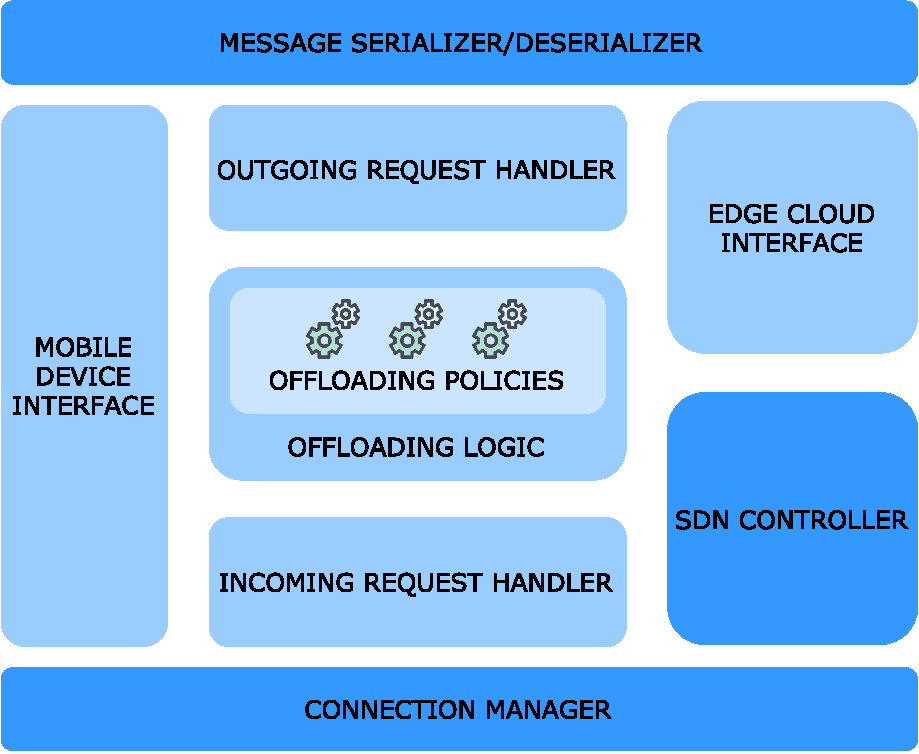
\includegraphics[width=0.8\textwidth]{img/off_sys_arch}
\caption{Offloading system architecture.}
\label{fig:offloading_system_arch}
\end{figure}

The main components are:
\begin{itemize}
\item a mobile device interface: interface for communications between the mobile devices and the offloading system
\item an edge cloud interface: interface for communications between the edge cloud and the offloading system
\item offloading logic: offloading policy to be used to serve the edge client
\item SDN controller: responsible of enforcing the offloading policies on the network devices.
\end{itemize}

The mobile device interface supports the communication between the mobile devices and the offloading mechanisms, providing a set of primitives necessary to the two parties to communicate efficiently and formalizes the offloading request requirements. The edge cloud interface has the same role of the mobile device interface, but the involved parties are different: in this case the primitives are meant for the communication between the offloading system and the edge cloud, but the objective remains the same. The offloading logic is the main part of the architecture, it contains the set of policies available as offloading criterion, allowing the mobile devices to specify which one they intend to use and users to implement their own. Finally, the architecture includes a SDN controller, that we believe, must be part of it, because of the numerous possibilities that SDN offers in terms of network management.  

\subsection{Offloading Protocol}
Through the edge and cloud interfaces, the parties communicate in order to complete a task offloading process. For this communication to happen, a protocol is required. In this context, the communicating parties are:
\begin{itemize}
    \item mobile device: sends request to the offloading server
    \item offloading server: accepts request from the mobile device, enforces the offloading policy by talking to the SDN controller and forwards the tasks to the edge server
    \item SDN controller: receives flows installation requests from the offloading server
    \item edge server: receives the tasks that need to be offloaded.
\end{itemize}

\begin{figure}[]
\centering
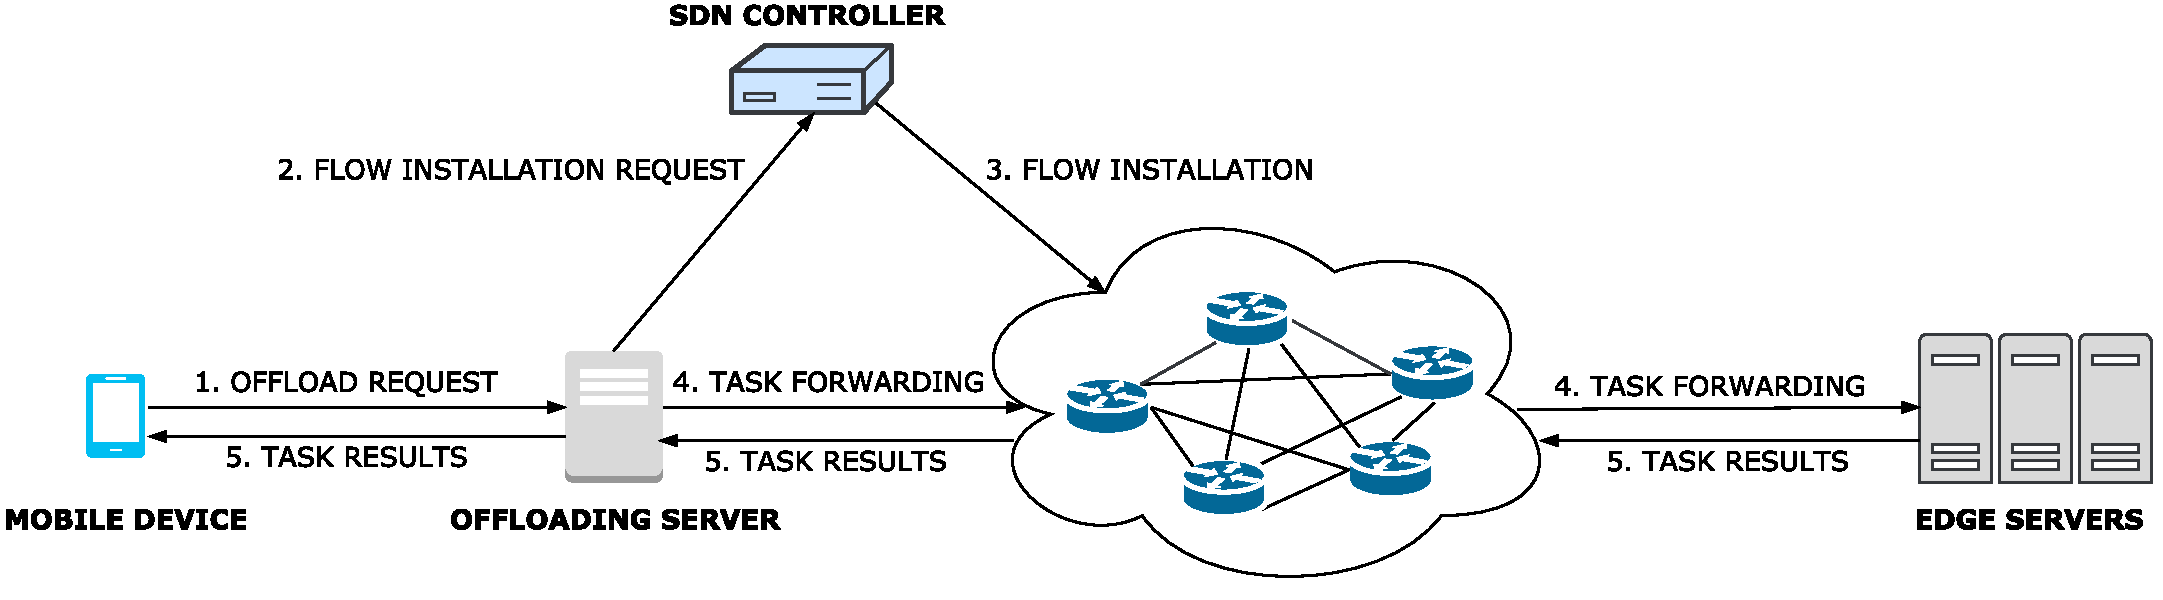
\includegraphics[width=\textwidth]{img/protocol_sequence}   
\caption{Offloading workflow: mobile devices and an offloading server orchestrate the request via an SDN controller}
\label{fig:protocol}
\end{figure}

Figure~\ref{fig:protocol} shows the typical message sequence needed to complete an offloading request; the required steps are the following:
\begin{enumerate}
\item the mobile device sends an offload request to the offloading server
\item the offloading server decides whether or not it is possible to accept the request and if so, where to offload it according to a set of configurable, i.e., programmable policies
\item the offloading server asks the SDN controller to install on the switches the flows required by the offloading policy~\footnote{This step is optional  because the required flows may be already installed}
\item the offloading server forwards the offloaded task to the edge server 
\item the edge server sends the computation result back to the offloading server, that in turn forwards it to the device.
\end{enumerate}

Task offloading is a complex problem, with a high number of factors involved in the final decision. In the literature, task offloading is also known as cyber-foraging~\cite{cyberforagingsurvey}. These factors include application requirements formalization, task retrieval, edge server/cloud discovery. Before explaining the details of our protocol (implementation), we describe some of these problems and how our protocol addresses them.\\\\
\textit{Application requirements formalization}

We assume that the application requirements are expressed in terms of \textbf{CPU ratio} (average CPU used to execute the task on the mobile device), \textbf{memory footprint} (quantity of memory required by the application) and desired \textbf{latency} (specifying if the task, is urgent or it can wait).\\\\
\textit{Task retrieval}

For the task retrieval problem we consider two different scenarios: in the first one the task is hosted on the server with the possibility to retrieve it with a unique identifier; in the second scenario, the task is sent to the server, wrapped in a container (e.g., a java package JAR or a python package EGG).\\\\
\textit{Edge servers discovery}

The implementation of a server discovering protocol is out of the scope of this project: we assume that the offloading server is aware of the available edge servers. Our implementation over mininet uses a Link Layer Discovery Protocol (LLDP).

\paragraph{Abstract Syntax Notation} 
With these assumptions in mind, we now describe the protocol messages definition using the Google Protocol Buffer~\cite{protobuf} abstract syntax notation; Google Protocol Buffer is a library that allows to easily specify structured messages through a \textit{.proto} file. The complete .proto file is available in the Appendix~\ref{proto_file} at the end of the report; what follows is a brief overview of the protocol main messages. An abstract syntax notation is necessary to provide computer architecture independence as well as programming language independent, and so to abstract out the implementation details. This means that users may use our .proto files to write their own server or client applications using for example, Java with a big-endian architecture for a server, and C++ with a little-endian computer architecture on the client. Historically, abstract syntax notations have been using ASN 1, and more recently, developers use XML or JSON. XML or JSON are however text-based, while Google Protocol Buffer is binary based, and so  serialize and deserialize messages  is more efficient with Google Protocol Buffer. An alternative could have been BSON, but Google Protocol Buffer provides already compilers for many languages so it has been our choice. We now describe the specifics of each message.

\paragraph{OffloadRequest} is the message sent from the mobile device to the offloading server and includes the requirements, the type of the task and optionally the task itself.

The \textbf{requirements} consist of the specification of the amount of cpu and memory necessary for the task to be executed and the level of latency needed. The idea of having a latency level allows a better support for real-time applications.

The \textbf{type} of the task is needed to support serverless computing~\cite{hendrickson2016serverless}~\cite{fox2017status} and implies two possible scenarios. In case of serverless computing the type of the task is set to \textit{LAMBDA} and it is assumed that the task is already on the server. If the type is set to \textit{STANDARD} then the code to be executed is sent as payload of the request.

The \textbf{task} could be an identifier (\textit{task\_id}) of the task on the edge server (in case of a lambda application), or the task itself. In the latter case, the executable and its type are included in the request in a message called \textit{TaskWrapper}.

\paragraph{Response} is a message used for several purposes; it is used to confirm the reception of a message or to signal an error. {\tt Response} is also used to send back to the mobile device the result of the computation. It is important to notice that protobuf messages are not self-delimiting, that means that it is necessary to know its size in order to receive it. Every time a new message needs to be sent, the sender starts with the message size first, if an OK response is received then the message is sent.

\paragraph{Message} is a wrapper for all the messages used in the system, its purpose is to ease the parsing process by having a \textit{type} field that can be one of the messages defined above.


\section{Path prediction via Deep Learning}
\label{sec:path_prediction}
\paragraph{Why Deep Learning?} Deep learning is currently one of the most active area of research. It has proven to be able to solve numerous problems in different fields, but it is not adopted to solve networking problem as much as in other contexts. In this work, we decide to use deep learning for two reasons: first of all, deep learning has shown great computation performance, especially for complex problems, furthermore, we want to understand if its poor adoption in networking is due to a lack of interest in the area or because it is not the right tool in this context. Before proceeding with this chapter, it is important to keep in mind that  the word deep in deep learning, is used every time a neural network has more than one layer. The architecture described in Section~\ref{sec:architecture} includes the \textit{offloading logic} block, responsible of determining the criterion on which the offloading is based. As a first offloading policy, we implement a deep learning model capable of finding the path towards a destination, that should be used in place of traditional routing policies. 

One of the problems of traditional routing algorithms is that they do not consider how the network load changes over time (they rely on TCP for congestion and flow control, and hence, by design they are performance-unaware): the path from a source to a destination is computed by taking into account static parameters, such as the nominal interface speed. This lack of consideration of the dynamic behavior of the network can cause traffic slowdown and packet loss in case of congestion, an undesired behavior in circumstances where latency is crucial. End-to-end congestion control when latencies are so important or when the network is so disruptive (in case of a natural disaster) is not enough. The intuition behind our project is that \textit{collaborative traffic steering} should be able to identify and avoid congestion situations, without using TCP or other active queue management approaches such as Explicit Congestion Notification (ECN). A collaborative policy requires, in some way, the participation of all the parties in the decision process, however, achieving nodes collaboration in a network is a complicated task. A simplified version of this collaborative mechanism could be the following: instead of all nodes being directly involved in the decision process, they could limit their role to notifying a central node of their current status. This is made possible by the SDN paradigm: in our system the nodes are connected to a SDN controller responsible of retrieving information about the nodes status, in this case using the OpenFlow protocol~\cite{openflow}. The information used in our system is the number of incoming packets on a node: the idea is that the packet distribution on the nodes, routers in this case, reflects the network conditions; a high packet count on a router is an indicator of a big load that is probably going to lead to packet loss and retransmission. Another point to clarify before proceeding with the implementation details, is that the distribution of packets on the routers is influenced by the routing algorithm: nodes that appear in multiple paths will probably have an higher count than less traversed nodes because they are responsible of forwarding packets for multiple source-destination pairs. If routers were able to see all possible outcomes of a routing protocol in a network and extract the consequent traffic patterns, they could try to choose the less busy path. This is exactly how we build our deep learning model: we simulate a small network with ten routers, we choose a routing algorithm (OSPF), we make it vary and record the traffic patterns. Afterwards, we use the collected data and the routing choices taken by the routing protocol to build a model capable of predicting each hop of the path, from the source to the destination. Learning from the algorithm we criticize and aim to replace may sound confusing and counterintuitive, but learning is different from copying. With our approach, we are correlating traffic patterns and routing decisions, replicating as many different scenarios as possible, so that the final model will have a complete view of the problem. The correlation between traffic patterns and routing allows are system to dynamically adapt to the network conditions, a behavior that wouldn't occur with a traditional routing algorithm. \\~\\For this problem, to create a working deep learning model, two elements are essentials: the dataset and the network architecture; the following sections describe the type of data, how we obtain them and what neural network architecture we select. 

\subsection{Dataset}
The performance of a machine learning model depends heavily on the data used to train it. Creating a working model requires having good data in terms of quantity and quality, namely the number of samples available to train the model and how well these samples represent the domain you are trying to model. Training a model with a dataset too small usually results in poor performance, because there are not enough information for the model to learn from, causing the system to deal with unknown scenarios; on the other hand, even a big dataset that only covers a small portion of the domain of study, will perform poorly because the system, will not be able to learn all of the different scenarios, therefore losing the ability to generalize and creating an abstraction. Ideally, the perfect dataset would be representative of the whole domain we are modeling.

Recently a lot of effort is being put in making datasets available to the machine learning community, with the aim of promoting research. In the context of networks, there is plenty of dataset available ~\cite{caida}\cite{fb_dataset}\cite{topo_zoo}; however those are mostly network captures of datacenters or small portions of networks, and they do not contain  details about the underlying topology nor the routing strategies. 

The elements needed to implement our path prediction system in a given a network are:
\begin{enumerate}
\item the network topology
\item the routing informations
\item the packet count on each node.	
\end{enumerate}
Since we could not find a dataset fit to our needs, we have created our own.

\subsubsection{Topology}
\label{sec:net_topology}
The first component of our system is the network: we need to emulate a network from which we can extract the data necessary to train the model and to use to test the final model. Mininet~\cite{mininet} is a software commonly used in the network virtualization research community, that can create a virtual network running real kernel, switch and application code with support for OpenFlow and Software-Defined Networking~\cite{openflow}.

Figure~\ref{fig:topology} shows the topology used in our system: it is composed of ten routers, R1-R6 which we denote from now on as \textit{outer routers}, and R7-R10, from now denoted as \textit{inner routers}. The topology includes also fourteen switches, the reasons of their presence is explained in section~\ref{sec:packet_counter}. For simplicity we assume that traffic is being generated only by the outer routers, therefore the inners' are only responsible of forwarding other nodes packets. The topology is a partially connected network with multiple paths connecting the same source-destination pair; note that having multiple paths is crucial for the path prediction system: in this way, during the training phase, our path prediction algorithm will learn several different alternative paths from source A to a destination B.

\begin{figure}[h]
\centering
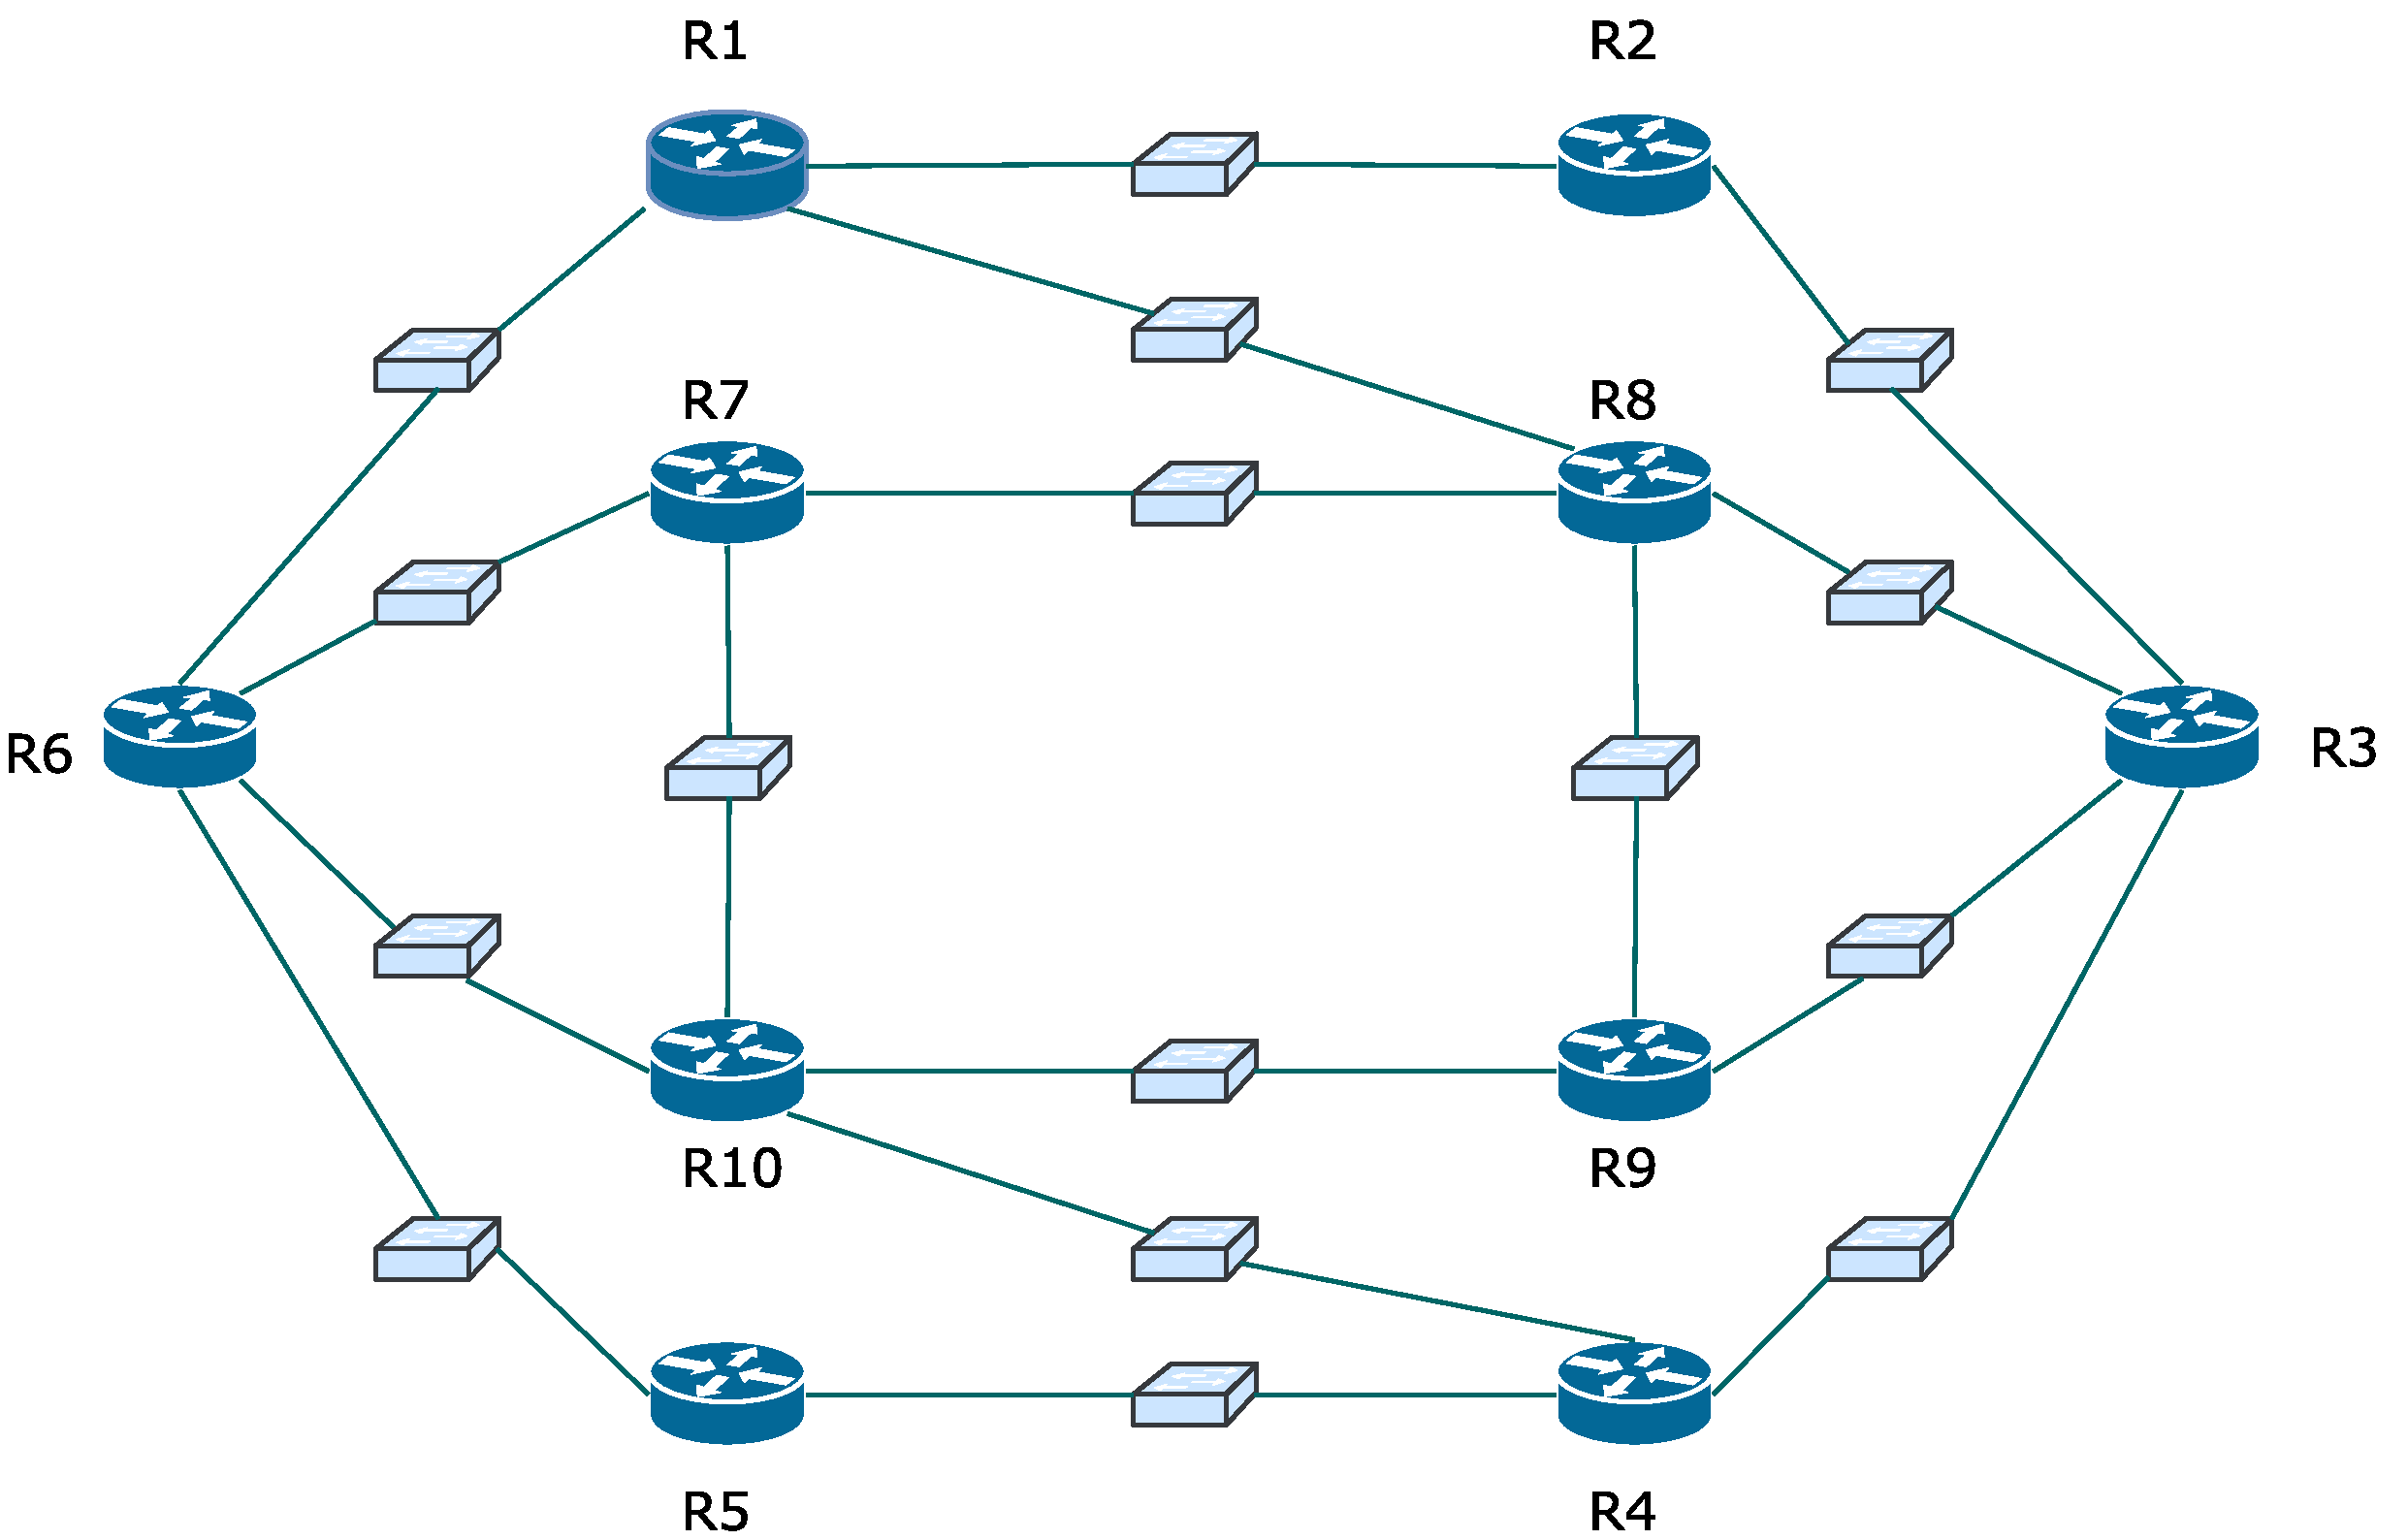
\includegraphics[width=\textwidth, keepaspectratio]{img/network_arch}
\caption{Model topology: R1-R6 are outer routers while R7-R10 are inner routers. Each router runs a next-hop predictor based on LSTM.} 
\label{fig:topology}
\end{figure}

\subsubsection{Routing information}
The default behavior of Mininet is to create a layer 2 topology, with all the nodes acting as a switch or a host in a local network. Our objective is to build a path prediction system that learns from the routing algorithms, hence we need to build a fully functional level 3 network with level 3 routers. The easiest way to use Mininet as a layer 3 network is through MiniNext~\cite{mininext}, a mininet extension layer that support routing engines and PID namespaces. As a routing engine we use Quagga~\cite{quagga}, a routing suite providing implementation of routing protocols for Unix platforms. The Quagga architecture consists of a core daemon, zebra, that acts as an abstraction layer to the underlying Unix kernel and presents the Zserv API over a Unix or TCP stream to Quagga clients. It is these Zserv clients which typically implement a routing protocol and communicate routing updates to the zebra daemon. MiniNext allows us to place routers into a mininet topology; the way it does this is by instantiating  a regular Mininet host node in a separate namespace and starting a routing process on it: different namespaces are necessary so that each host can run the routing process without interfering with the others. Figure~\ref{fig:quagga_mininext} shows an outline of this architecture: each Mininet host runs in a separate namespace and runs the zebra and the routing daemons; each zebra daemon updates each router routing table with the routing informations exchanged through the virtual network built with the Linux Kernel.

\begin{figure}
\centering
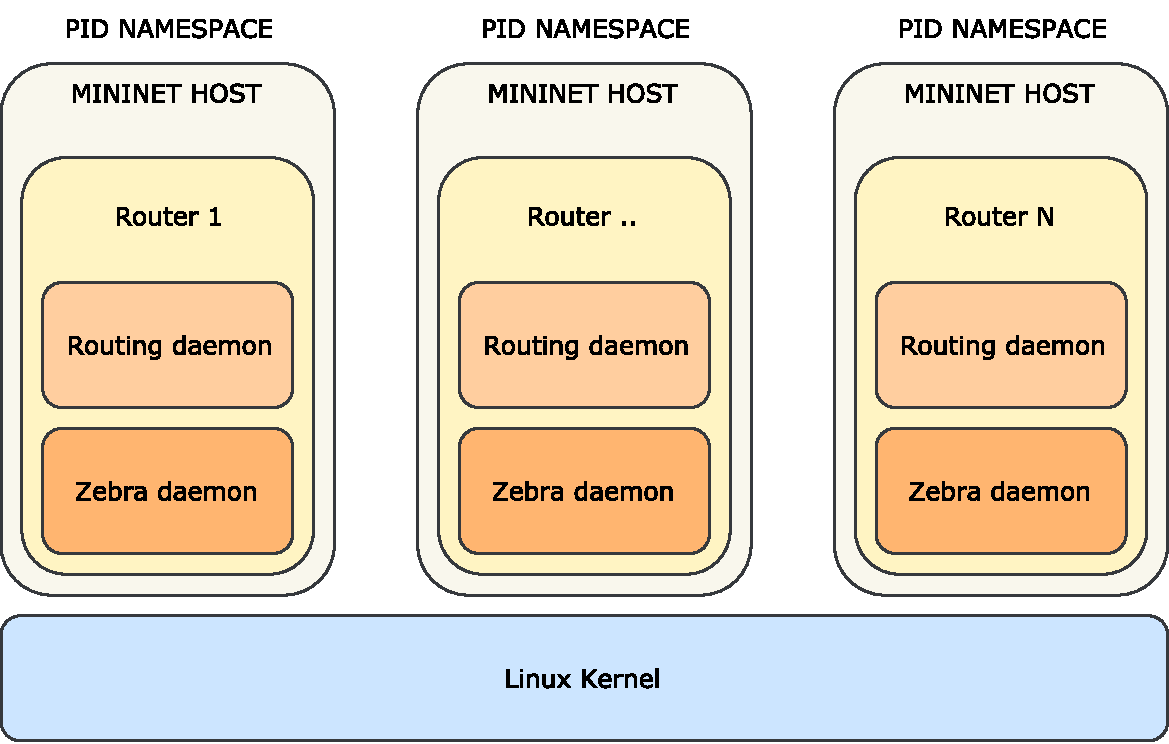
\includegraphics[width=\textwidth]{img/quagga_mininext}
\caption{Quagga router implementation in MiniNext.}
\label{fig:quagga_mininext}
\end{figure}

\subsubsection{Router packet counter}
\label{sec:packet_counter}
In section~\ref{sec:net_topology} we have described the topology without giving an explanation of the presence of a switch between every pair of connected routers. The reason for the switches is that we want this system to work in a SDN context: the only way to use a SDN controller in Mininet is to use switches. There is also a secondary reason that justifies the switches presence: unlike the routers, switches do not run in a separate namespace, allowing traffic analyzer tools such as Wireshark to capture traffic on all the network interfaces at once. Because of the separate PID namespaces, if we wanted to capture traffic directly on the routers interfaces we would need a Wireshark instance for each router, that would make debugging extremely hard. 

An SDN controller can retrieve switches information with the OpenFlow protocol; in this project we use Ryu~\cite{ryu}, an SDN controller written in Python. Since the controller is connected to the switch, getting the packet count on the router is not trivial. On an OpenFlow enabled switch it is possible to get the number of packet received on each port; given that each router is directly connected to at least one switch, it is possible to infer the number of packets directed to the router by counting the number of packets coming from a certain port of the switches it is connected to. Figure~\ref{fig:packet_counter} explains this concept with an example: in the figure, the number of incoming packets on R1 at a given time is the sum of the incoming packets on port1 of S1 and port2 of S2. By repeating this procedure for all the routers in the network, the controller is capable of retrieving, at any given time, the number of incoming packets on each router.
\begin{figure}[h]
\centering
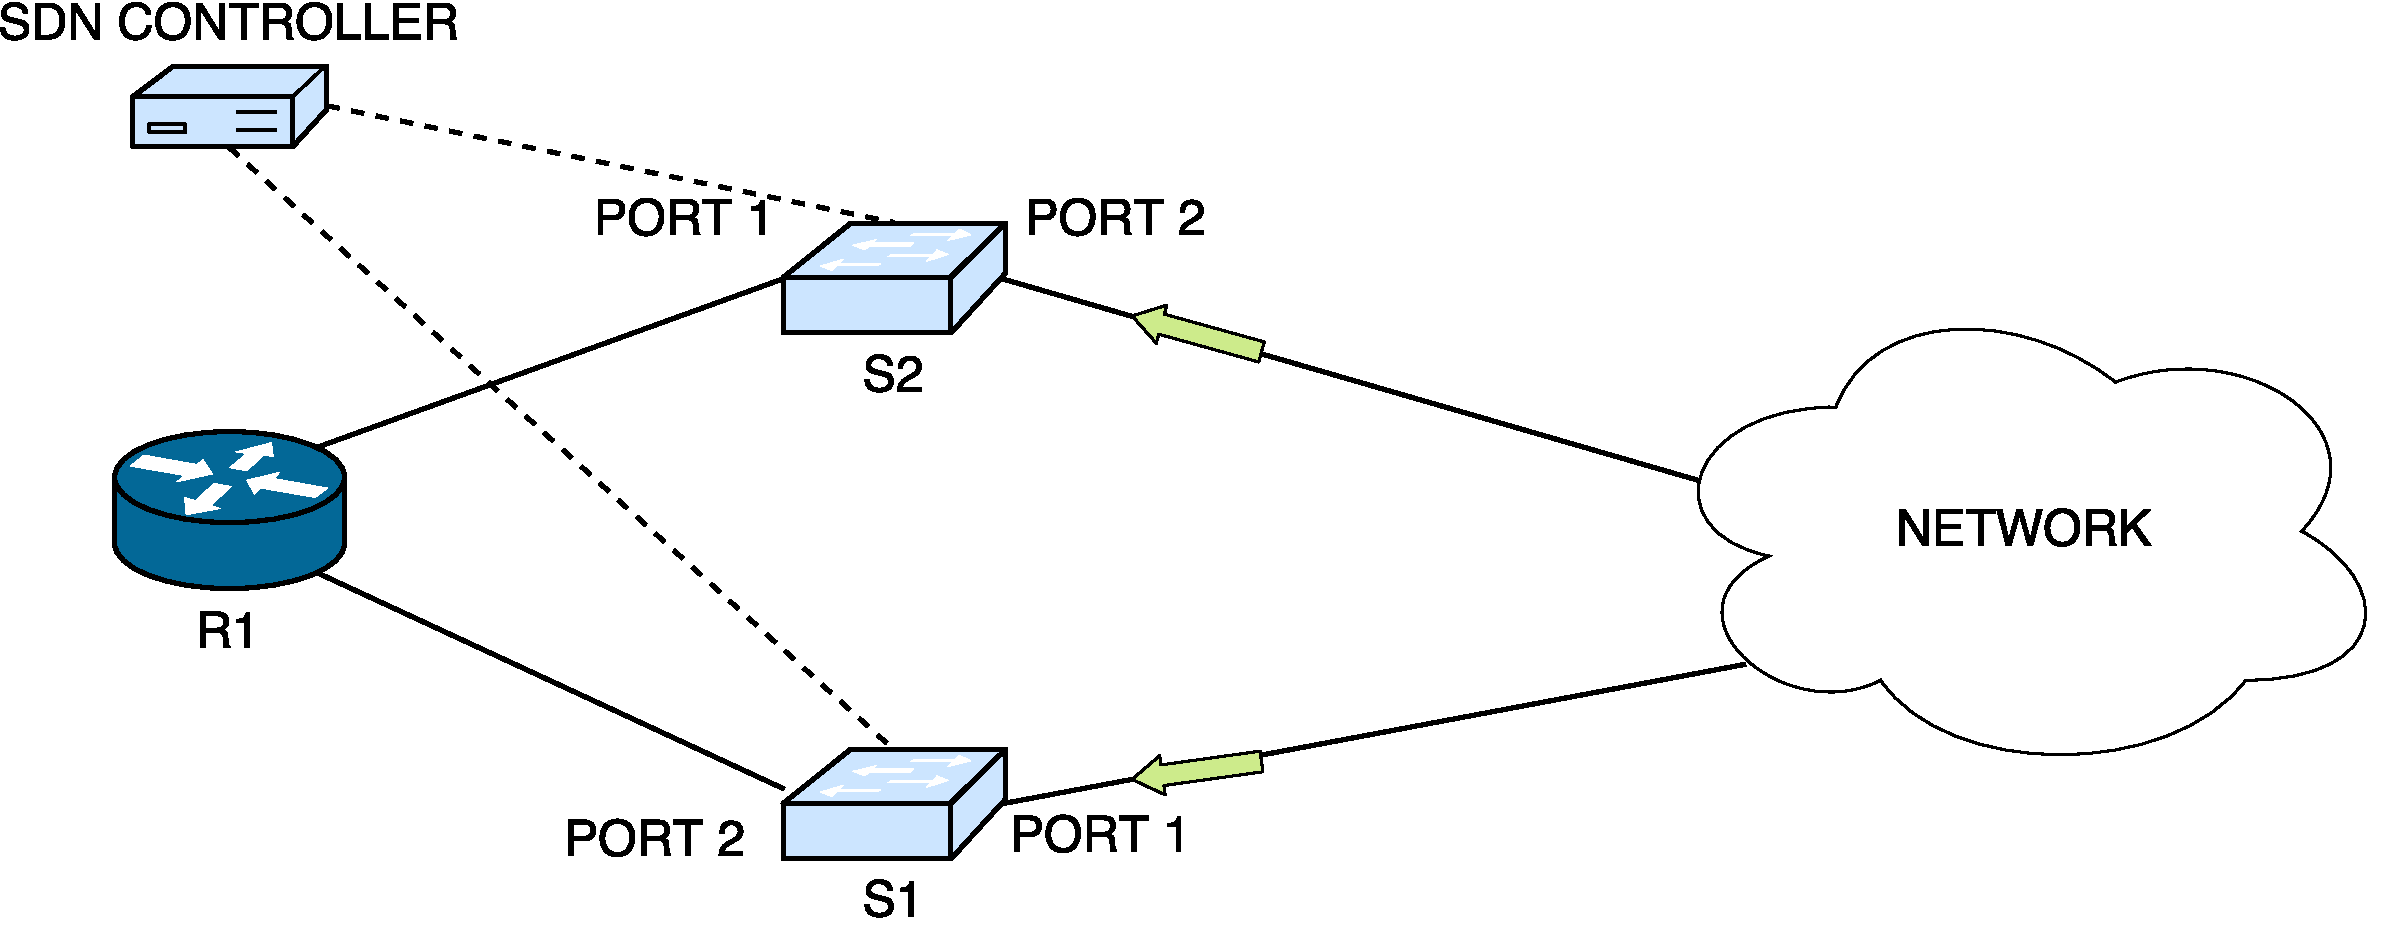
\includegraphics[width=\textwidth]{img/packet_counter}
\caption{Router packet counter explanation}
\label{fig:packet_counter}
\end{figure}

\subsubsection{Dataset Generation}
Up to this point we have a fully functional level 3 network, with a running instance of the OSPF routing protocol, connected to a controller capable of retrieving the packet count on each router when needed. To build our system we need a set of labeled data from which the model can learn. More specifically, we need a collection of samples containing at a given time, the packet counting information together with the routing information. The detail about the data format and how they are used are described in the following section~\ref{sec:dl_model}; in the rest of this paragraph we describe how we generate these data.

The idea is to simulate the traffic conditions in a regularly functioning network, collect the traffic and routing information, and use it to train the network. By default, a mininet network is static, in the sense that there is no traffic unless manually generated. One way to generate traffic is by using \textit{iperf}~\cite{iperf}, a tool for bandwidth measurement in IP networks. As a second step, we need to change the output of OSPF over time to explore the various paths in the network. OSPF computes each path cost according to the speed of the network interface; therefore,  changing such speed is sufficient to force OSPF to compute new routes. 

We generate our training dataset as follows: for \textit{ospf\_configurations} times, every \textit{ospf\_conf\_duration} seconds, the network is teared down and rebuilt with a new link speed, producing a new OSPF configuration; for each OSPF configuration, traffic is generated in the network by running the \textit{iperf} Linux utility between every source-destination pair, with a certain \textit{transmission\_probability} and a \textit{transmission\_time} duration. In the meantime, the controller retrieves the packets count every \textit{sampling\_time} seconds and saves it to a file, while another script saves the routing tables of each router, every time that the OSPF configuration changes. The pseudo-code of the algorithm is shown in Figure~\ref{fig:traffic_gen} while table~\ref{tab:dataset_params} describes the algorithm parameters.

\begin{algorithm}[t]
\captionof{figure}[Traffic generation algorithm]{Traffic generation algorithm}
\label{fig:traffic_gen}
\begin{algorithmic}
\FORALL{\textit{ospf\_configurations}}
	\FORALL{\textit{(src, dst) pairs}}
		\STATE{$p=random(0, 1)$}
		\IF{$p<transmission\_probability$}
			\STATE{$t=randint(0, transmission\_time)$}
			\STATE{\textit{run iperf for t seconds}}
		\ENDIF
	\ENDFOR
\ENDFOR
\end{algorithmic}
\end{algorithm}

\begin{table}[b]
\resizebox{\textwidth}{!}{%
	\begin{tabular}{|l|c|l|ll}
	\cline{1-3}
	\multicolumn{1}{|c|}{\textbf{Parameter}} & \textbf{Value} & \multicolumn{1}{c|}{\textbf{Description}}                        &  &  \\ \cline{1-3}
	\textit{ospf\_configurations}            & 15             & number of different OSPF configurations                   &  &  \\ \cline{1-3}
	\textit{ospf\_conf\_duration}            & 20 m           & time after which a new ospf configuration is produced            &  &  \\ \cline{1-3}
	\textit{transmission\_probability}       & 0.65           & probability with which there is traffic between a pair of routers &  &  \\ \cline{1-3}
	\textit{transmission\_time}              & 0-5 s          & time in seconds to transmit for (iperf)                          &  &  \\ \cline{1-3}
	\textit{sampling\_time}                  & 1 s            & sampling time of the packet count                                &  &  \\ \cline{1-3}
	\end{tabular}%
	}
\caption{Dataset generation parameters.}
\label{tab:dataset_params}
\end{table}

Using the parameter set of table~\ref{tab:dataset_params}, we obtain a dataset of 17696 samples; 85\% of these samples form the training set, and the remaining 15\% is used as test set.

\subsection{Deep Learning Model}
\label{sec:dl_model}
The deep learning model chosen for this project is a LSTM, a Recurrent Neural Network (RNN): recurrent neural networks are a class of neural networks in which connections between nodes form a directed cycle (Figure~\ref{fig:rnn}). These connections allow the nodes to memorize information about what has been computed so far. The reason we choose RNNs is because of their ability to make use of sequential information and to exhibit a dynamic temporal behavior. We wanted our model to learn the correlation between changes in the packet distribution and routing decisions over time.

So far we have discusses our machine learning model as if a single instance would be able to  predict every path for every possible source-destination pair; however, given the complexity of routing, this scenario did not seem feasible. Our solution is to train a separate model for every $(s,d)$, resulting in several simpler models rather than a single, very complex one. To give an idea of the order of magnitude of this approach, a network with $N$ nodes will result in $N(N-1)$ models. These numbers need to be adjusted if each node has, like in our case, more than one network interface; in this scenario, there will be more models with respect to the previous case, each one describing a particular $(src\_router, dst\_address)$ pair.

\begin{figure}[]
\centering
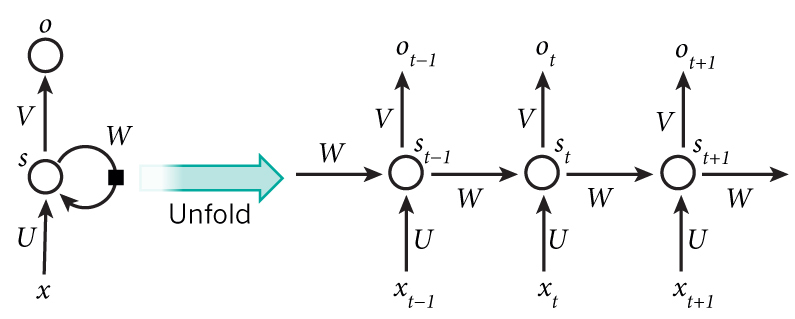
\includegraphics[width=\textwidth]{img/rnn}
\caption{Recurrent neural network and its unfolded version.\protect\footnotemark }
\label{fig:rnn}
\end{figure}
\footnotetext{Picture from:~\url{http://www.wildml.com/2015/09/recurrent-neural-networks-tutorial-part-1-introduction-to-rnns/}}

\subsubsection{Input/Output modeling}
A machine learning model requires a proper representation of the input and output; supervised learning involves a sample space $X$ and a label space $Y$, with the network responsible of learning a mapping function from values in $X$ to labels in $Y$, for each $(x_i, y_i) \in X\times Y$. Our input/output modeling follows the same approach described in~\cite{Kato}: given $O$ the set of outer routers, and $R$ the set of all the routers in the network, for each $(s, d) \in R \times O$, the system learns the next hop for that particular target destination. Note that the fact that inner routers are included in the set of sources nodes is not a conflict with what stated in~\ref{sec:net_topology}: even though these routers do not generate traffic, they are still responsible for forwarding packets coming from other sources.

{\bf Each model learns the next hop for a particular destination, given the packet count on each router at a given time $t$: } the easiest way to model the input is an $N$\textit{-dimensional} array, with N being the number of routers in the network. The array is indexed by the router number, so the \textit{i-th} element of the array is the number of incoming packets on router \textit{i}. The output is modeled as a one-hot encoded, router indexed array, with a 1 in the position indexed by the predicted next hop; the size of the output is again equal to the number of routers in the network.

\subsubsection{Neural Network Architecture}
The architecture of a deep neural network is determined by the number of layers, the number of processing units (neurons) per layer and the interconnections between the layers. Choosing these parameters once at the beginning, hoping to achieve good performance, is not feasible given the impossibility to derive them from a formal description of the problem; thus, these parameters need to be tuned in a preliminary phase. As a general rule, a network too small will not be able to solve the problem and a network too big will probably overfit on the training set; there is also consensus on the fact that for the majority of the problems, adding additional hidden layers does not significantly improve the performance.

To define the parameters of our network, we follow these three steps:
\begin{enumerate}
\item pick a source-destination pair that requires a complex model
\item cross-validate each combination of layer and neurons
\item choose the combination whose accuracy -- loss pair is best.
\end{enumerate}

It is important to clarify what we mean with \textit{``source-destination pair that requires a complex model``}: cross-validating the different architectures on all the possible pairs would be excessively time-consuming, thus we decide to perform the validation on a single target. From now on, a target is simply a source-destination pair. For this validation to be meaningful, we need our target to be representative enough of the problem we are modeling: since we want our system to learn alternative paths, it would not make sense to choose a target of two directly connected nodes, because the resulting model would be too simple. As a consequence, we choose the target $(R1, R4)$; Figure~\ref{fig:validation_target} illustrates some of the 3-hop paths connecting the two routers.

\begin{figure}[]
\centering
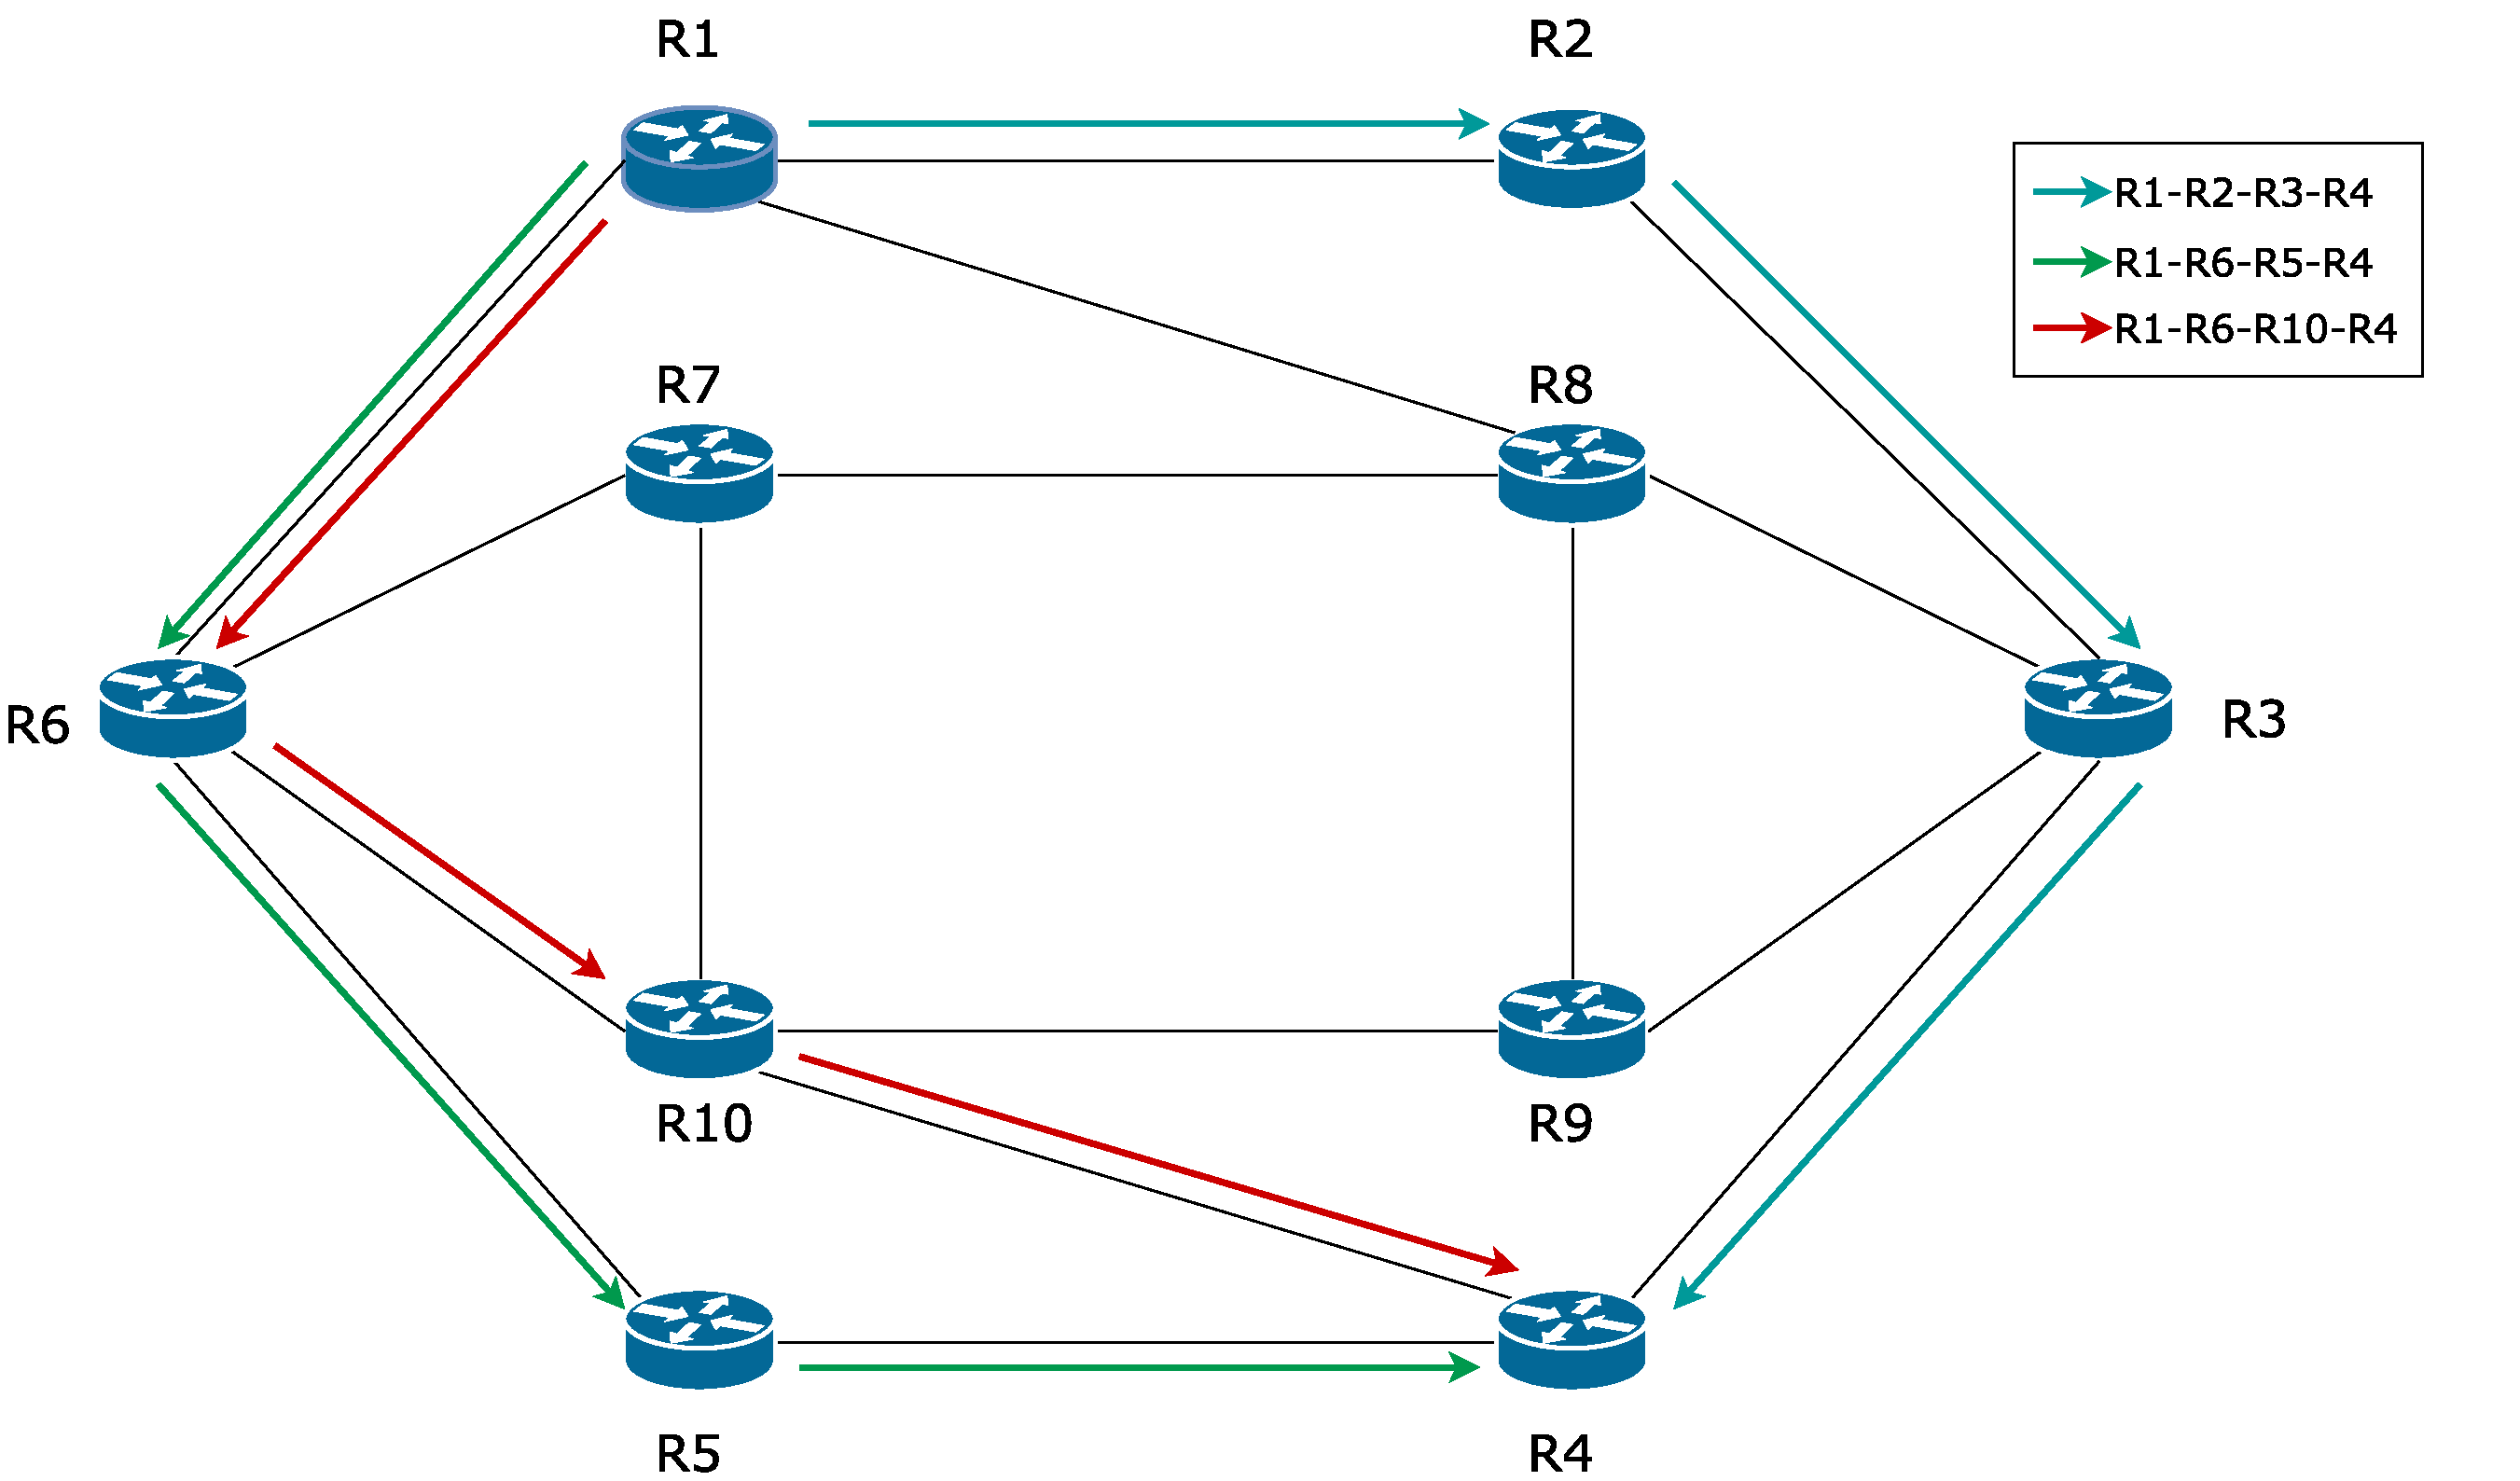
\includegraphics[width=\textwidth]{img/validation_target}
\caption{Examples of paths connecting the validation target.}
\label{fig:validation_target}
\end{figure}

As it is noticeable from the figure, there are several paths with the same number of hops connecting the two routers, so, in the context of choosing a representative model, the selected target seems a good candidate.

In the cross-validation phase, we test 24 different configurations by trying all the combinations of the following parameters:
\begin{itemize}
\item $hidden\_layers=\{2,4,6,8\}$
\item $neurons=\{4, 8,16,32,64,128\}$.
\end{itemize}

It is important to remind that each hidden layer is a recurrent layer with LSTM cell.
Each configuration is tested 10 times on different partitions of the dataset, producing the results in table~\ref{tab:arch_results}. The table shows two metrics: accuracy (percentage of samples correctly classified) and cross-entropy loss (distance between predicted and true label distribution); it is evident that what we described earlier about how adding layers does not significantly improve the performance, applies in this case. All the noticeable improvements in the results are caused by increasing the number of neurons in each layer (as you may notice by reading the table line by line); instead, if you read the table column wise (fixed number of neurons and increasing number of layers), you will not notice any performance gain. A 4-layers 128-neurons achieves the best performance in terms of accuracy whereas a 4-layers 128-neurons has the lowest loss; it is worth noticing that overall, given a fixed number of neurons, the performances typically differ by less than $1\%$ in accuracy. 

\begin{table}[]
\centering
\resizebox{\textwidth}{!} & \textit{Loss} & \textit{Accuracy \%} & \textit{Loss} & \textit{Accuracy \%} & \textit{Loss} & \textit{Accuracy \%} & \textit{Loss} & \textit{Accuracy \%} & \textit{Loss} & \textit{Accuracy \%} & \textit{Loss} \\ \hline
2 & 86.59\% & 0.5147 & 88.82\% & 0.3946 & 92.95\% & 0.3026 & 94.85\% & 0.2159 & 95.60\% & 0.1659 & 96.08\% & 0.1368 \\ \hline
4 & 76.48\% & 0.6416 & 87.69\% & 0.4644 & 92.99\% & 0.2435 & 94.90\% & 0.2045 & 95.70\% & 0.1554 & \textbf{96.58\%} & 0.1214 \\ \hline
6 & 64.90\% & 0.7727 & 88.82\% & 0.4450 & 92.72\% & 0.2515 & 95.25\% & 0.1663 & 95.38\% & 0.1541 & 96.14\% & \textbf{0.1149} \\ \hline
8 & 65.84\% & 0.7953 & 87.42\% & 0.4914 & 91.01\% & 0.3340 & 95.08\% & 0.1718 & 95.83\% & 0.1374 & 95.73\% & 0.1361 \\ \hline
\end{tabular}%
}
\caption{LSTM architectures comparison.}
\label{tab:arch_results}
\end{table}

From this first analysis it is clear that to achieve the best accuracy, each layer of the network needs to have 128 processing units; however, deciding what is the optimal the number of layers is a challenging problem. Since the gain in performance with an increase of the number of layers is not noticeable, we decided to take into account other factors to choose the final architecture. Table~\ref{tab:arch_timing} shows the average training time for the different configurations: in this case the impact of additional layers is evident. The training time seems to vary linearly with the number of layers: if we double the layers we basically double the training time.
Figure~\ref{fig:timing_cmp} compares the different training times with the model performance in terms of accuracy;
it is clear that while the training time increases noticeably with additional hidden layers, the gain in accuracy is barely noticeable and sometimes inexistent. Considering the limited computational power and time, and the number of models we need to train, we decide to use a network with 2 layers and 128 neurons, as a good trade-off between performance and time.

\begin{table}[]
\centering
\begin{tabular}{|c|c|c|c|c|c|c|}
\hline
 & \multicolumn{6}{c|}{\textbf{Neurons}} \\ \hline
\textbf{Layers} & 4 & 8 & 16 & 32 & 64 & 128 \\ \hline
2 & 301.20 s & 304.82 s & 314.56 s & 326.72 s & 388.46 s & 623.84 s \\ \hline
4 & 487.49 s & 499.91 s & 516.06 s & 557.60 s & 675.94 s & 1129.96 s \\ \hline
6 & 686.25 s & 705.11 s & 722.09  s & 781.28 s & 961.83 s & 1649.99 s \\ \hline
8 & 905.18 s & 931.16 s & 972.52 s & 1029.73 s & 1275.34 s & 2121.93 s \\ \hline
\end{tabular}
\caption{LSTM architectures average training time.}
\label{tab:arch_timing}
\end{table}

\begin{figure}[]
\centering
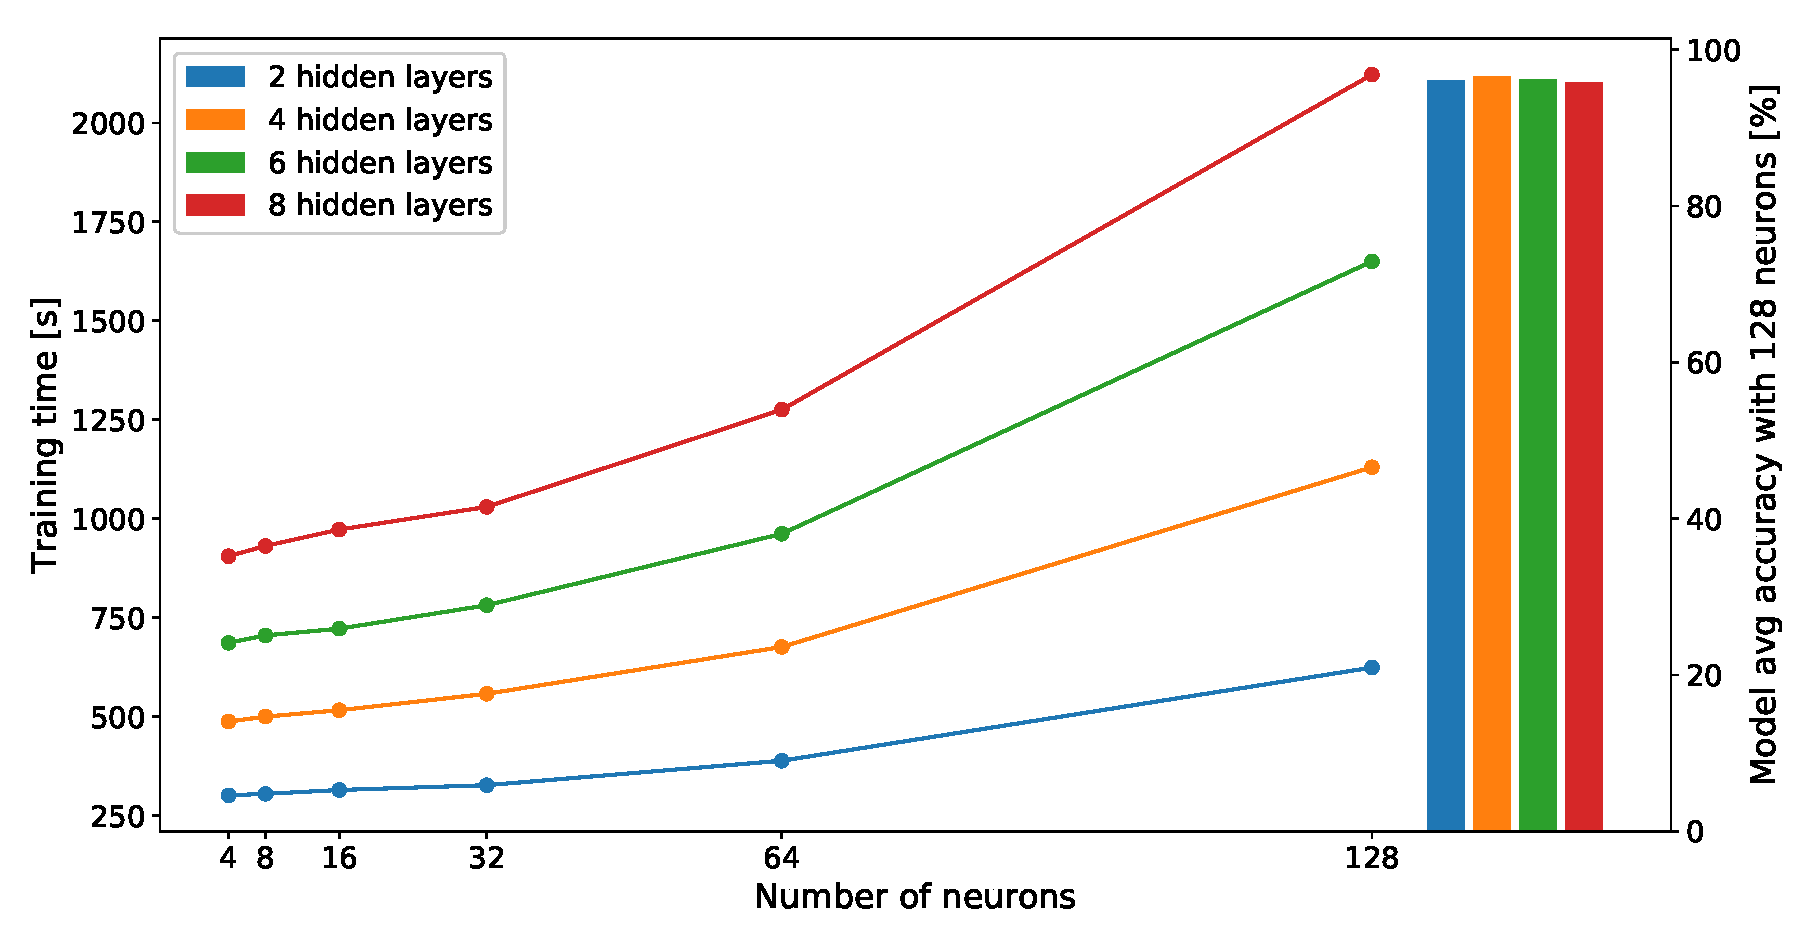
\includegraphics[width=	\textwidth]{img/timing_cmp.eps}
\caption{Comparison between training time and accuracy for 128 neurons.	}
\label{fig:timing_cmp}
\end{figure}

As a result of this analysis, the final architecture is composed as follows:
\begin{itemize}
\item input layer (10 neurons)
\item two hidden layers (128 neurons ea., hyperbolic tangent activation~\footnote{\label{fn:activation_fun}The activation function defines the output of a node given an input~\cite{Goodfellow-et-al-2016}})
\item output layer (10 neurons, sigmoid activation~\footnoteref{fn:activation_fun})
\end{itemize}

\noindent
{\bf Challenges of training a neural network.}
When training a neural network, there are some precautions necessary to avoid problem such as overfitting and increase training efficiency, avoiding exploding and vanishing gradient problems. Input normalization is the process of transforming all variables in the input data to a specific range, typically scaling the inputs to have mean 0 and a variance of 1, in order to have the same range of values for each of the inputs, guaranteeing stable convergence of the network weights and biases. Regularization is a technique to prevent overfitting, that  is characterized by adding a regularization term to the loss in order to prevent the weights to fit perfectly to the training data,  so that over all model is much more generalized. Dropout~\cite{srivastava2014dropout} is another technique to address the overfitting problem; the idea is to randomly drop units and their connections from the neural network during training, to prevent units from co-adapting too much.
In our case, we apply a batch normalization layer on the input, dropout on both the recurrent and feed-forward connections, and $L2$ regularization to the loss function. Figure~\ref{fig:normalization_cmp} shows the impact of normalization on the training performance: for both accuracy and loss, the normalization layer dramatically improves the performance, with a gain of about the 20\%.

\begin{figure}[]
\centering
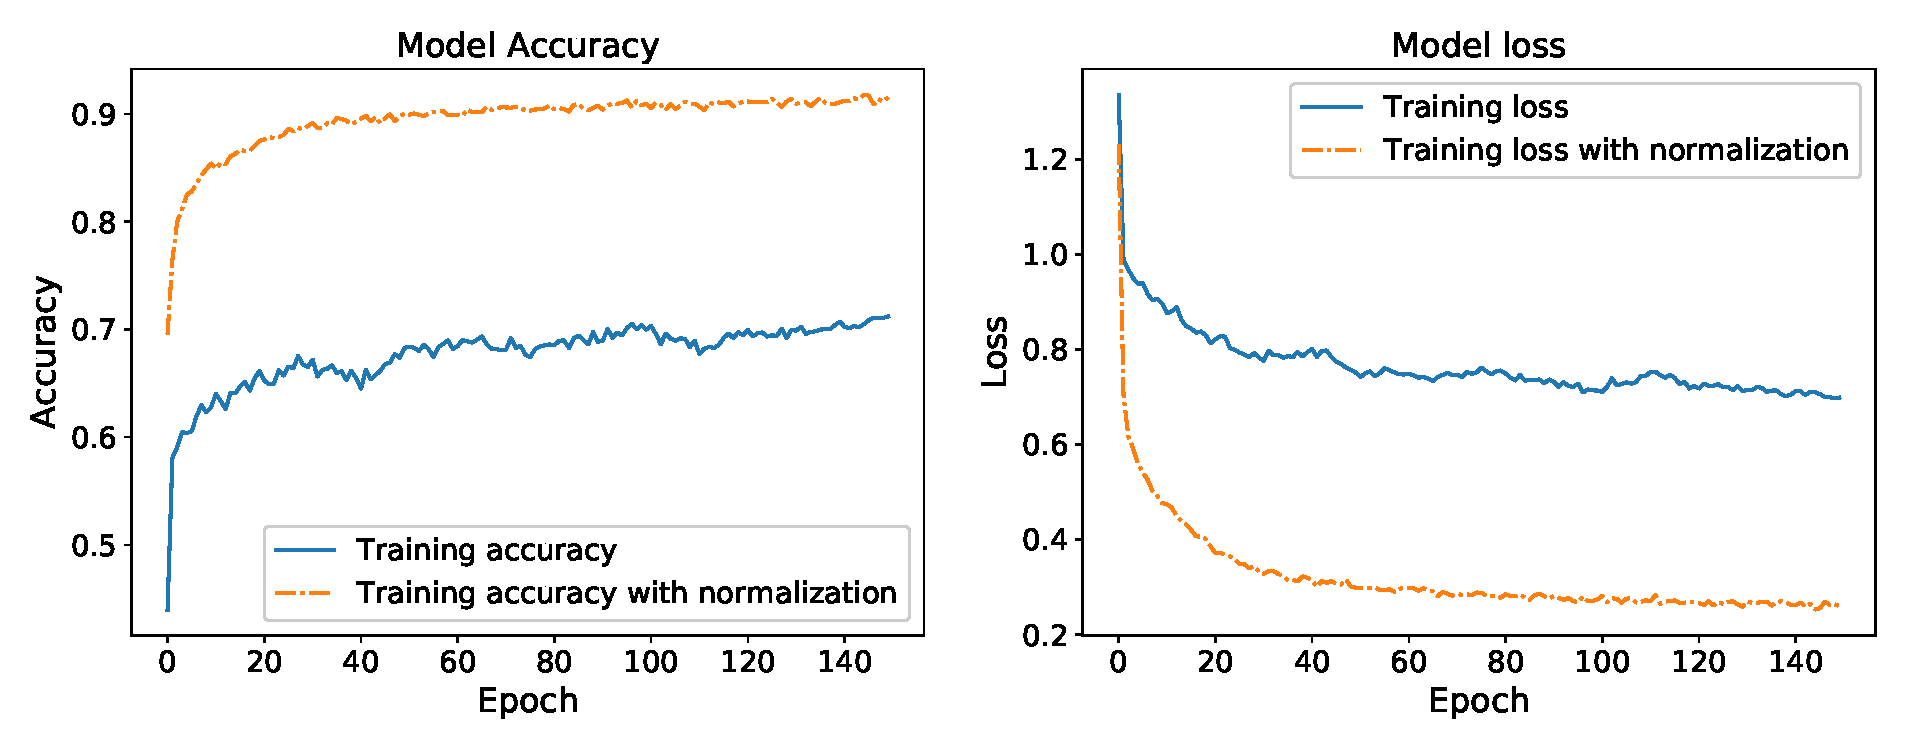
\includegraphics[width=\textwidth]{img/normalization_cmp}
\caption{Impact of input normalization on training accuracy and loss.}
\label{fig:normalization_cmp}
\end{figure}

\section{Implementation}
\label{sec:implementation}
To prototype our system we use the following tools:
\begin{itemize}
\item Ryu: SDN controller written in Python~\cite{ryu}
\item Google Protocol Buffer: framework for serializing structured data~\cite{protobuf}
\item Mininet: virtual network creation tool~\cite{mininet}
\item Quagga: routing software suite~\cite{quagga}
\item Keras: high-level neural networks API written in Python~\cite{keras}
\item Tensorflow: as Keras backend for the deep learning implementation~\cite{tensorflow}
\end{itemize}
%!TEX root = tesi.tex
\chapter{Related Work}
\label{ch:related_work}
In this chapter we describe the works related to this project, the relevant topics are cyber-foraging or task offloading, and machine learning applied to networking.\\\\
Cyber-foraging is a highly complex problem since it requires to take into consideration multiple issues. Lewis and Lago~\cite{catalog} dive into those issues and present several tactics to tackle them. Tactics are divided in \textit{functional} and \textit{non-functional}, with the former identifying the elements that are necessary to meet Cyber-foraging requirements and the latter the ones that are architecture specific. Functional tactics cover computation offload, data staging, surrogate provisioning and discovery; non-functional tactics deal with resource optimization, fault tolerance, scalability and security. They describe a simple architecture which include an \textit{Offload Client} running on the edge device and an \textit{Offload Server} running on the surrogate (cloud or local servers).

Wang et. al~\cite{edge_cloud_offloading_undersubmission:} report the state-of-the-art efforts in mobile offloading. More than ten architectures are described, each one in a different possible offloading situation. In particular the reported works face the single/multiple servers as offloading destination scenario, the online/offline methods for server load balancing, the devices mobility support, the static/dynamic offloading partitioning and the partitioning granularity.

In the last few years machine learning is being used to solve various challenges but it is not being widely adopted in networking problems; however, many people are trying to change this tendency. Malmos~\cite{malmos} is a mobile offloading scheduler that uses machine learning techniques to decide whether mobile computations should be offloaded to external resources or executed locally. A machine learning classifier is used to mark tasks for local or remote execution based on application and network information. To handle the dynamics of the network an online training mechanism is used so that the system is able to adapt to the network conditions. Malmos has proven to have higher scheduling performances than static policies under various network conditions.

The problem of resource management can be effectively addressed with machine learning~\cite{mao2016resource}. Generally speaking, resource management is a complex task that requires appropriate solutions depending on the workload. The authors implement a job scheduler based on Reinforcement Learning (RL); the results show a system that performs comparably to state-of-the-art heuristics, responsive to different conditions and with fast convergence.

Machine learning is also being used for computation offloading in mobile edge networks~\cite{crutcher2017hyperprofile}. Regression is used to predict the energy consumption during the offloading process as well as the time to for the access point to receive the payload. Available servers are represented in a feature space according to a hyper-profile, then K-NN (K-nearest neighbor) is used to determine the closest server based on metrics related to the hyper-profile. By using K-NN, if an application needs to partition a task into multiple parts onto multiple servers, one should simply vary the value of K. 

Kato et. al~\cite{deep_learning_heterogeneus} show the use of deep learning techniques for network traffic control. A DNN (deep neural network) is used for the prediction of a router next hop. The decision is based on the number of inbound packets in a router at a given time and OSPF paths are used for training. By combining the next hop decision for each router the system is able to predict the whole path from source to destination. Results show that the system is able to improve performances in terms of signaling overhead, throughput and average per hop delay with respect to the classic OSPF algorithm.

Another use of machine learning in networking is described in~\cite{end-to-end}. Bui, Zhu, Pescapé \& Botta designed a system for a long horizon end-to-end delay forecast. The idea is to use measured samples of end-to-end delays to create a model for long horizon forecast. Considering the set of samples as a discrete-time signal, wavelet transform is applied which results in two groups of coefficient. A NN (neural network) and a K-NN classifier are then used to predict the coefficients. Once again ML techniques seem to provide good results when applied to networking.

Valadarsky et al.~\cite{Valadarsky} discuss the advantages of a data-driven approach to routing, using two different machine learning techniques, in an intradomain routing case study. Two scenarios are considered: learning future traffic demands from past patterns or learning optimal routing configuration. To predict traffic demands supervised learning is used, on the other hand, for the prediction of routing configurations, the idea is to use reinforcement learning. The results show that while supervised learning might be ineffective are irregular, reinforcement learning is much more promising to generate effective routing configurations.
%!TEX root = tesi.tex
\chapter{Results}\label{ch:results}

In this chapter we evaluate the path prediction system; first we describe how our system can emulate OSPF by analyzing the results of the model training; finally we discuss the performance of the path prediction model as a substitute to more traditional routing algorithms. For a more complete analysis, we also implement the same Deep Neural Network (DNN) described in \cite{Kato}, a traditional neural network with four hidden layers and sixteen neurons in each layer. We use this network to compare the performance between DNNs and LSTM for the same task and understand if our hypothesis about RNNs is correct.

\section{Learning from OSPF}
Our system is built to learn the  behavior of OSPF across different configurations, and correlate it with different traffic patterns. We use a LSTM RNN as a learning algorithm and build a model for each source-destination pair in our topology (Figure~\ref{fig:topology}): the total number of models is given by all the possible source-destination  pairs, with the destination addresses considered only on the outer routers not considering the source; for any given a router, the number of addresses associated to it is equal to the number of its interfaces. In our considered scenario, this resulted into a set of $162$ distinct models that are used to determine the hop-by-hop path from a source router to a specific destination address. The path is computed iteratively as follows: starting from the source, the model for the selected destination is used to predict the next hop, then the predicted next hop becomes the new source router; the process is then repeated until the predicted hop is the final destination. Given their significant size, it is unfeasible to analyze all models individually; we are interested in exploring the overall performance. To do so, we analyze the average accuracy and loss over all different models, as discussed in the previous chapter.

Figure~\ref{fig:training_avg} shows the model training progress over time in terms of accuracy and loss: the plot shows the average of the metrics over all $162$ models. The slopes of the graphs give us an idea of what is happening during the training phase: at the beginning (epochs 0-20), both slopes are very steep, indicating that the model is abandoning the initial randomness and converging towards a final stable solution. Afterwards, from epoch 20 to 60, as the gradient diminishes, the slope starts to decrease slowly, indicating that the gradient has probably entered the region of the space in which it will converge to the problem solution. Finally, the curve becomes almost flat, showing that the gradient has reached its  minimum. Note how in both graphs, the two curves have the same behavior: this shows that the model is learning ``without losing generalities``. An increasing accuracy on the training set with a steady or decaying validation accuracy would be a clear sign of overfitting, a situation in which the model becomes too specialized on the training data and it is not able to properly classify new samples. 
The figure shows better performance for both accuracy and loss on the validation data rather than on the train data; even if generally unusual, the reasons of this behavior can be found in the dropout regularization technique. At training time, because of dropout, only part of the network is used; on the other hand, when testing the development of the model on the validation set, regularization mechanisms (i.e., dropout) are turned off, so the network is used in its completeness. This means that the whole network is used to measure accuracy and loss on the validation set but only a part of it is used for the same metrics at training time: for this reason, the performance on the validation set are slightly better than on the training set. 


\begin{figure}
\centering
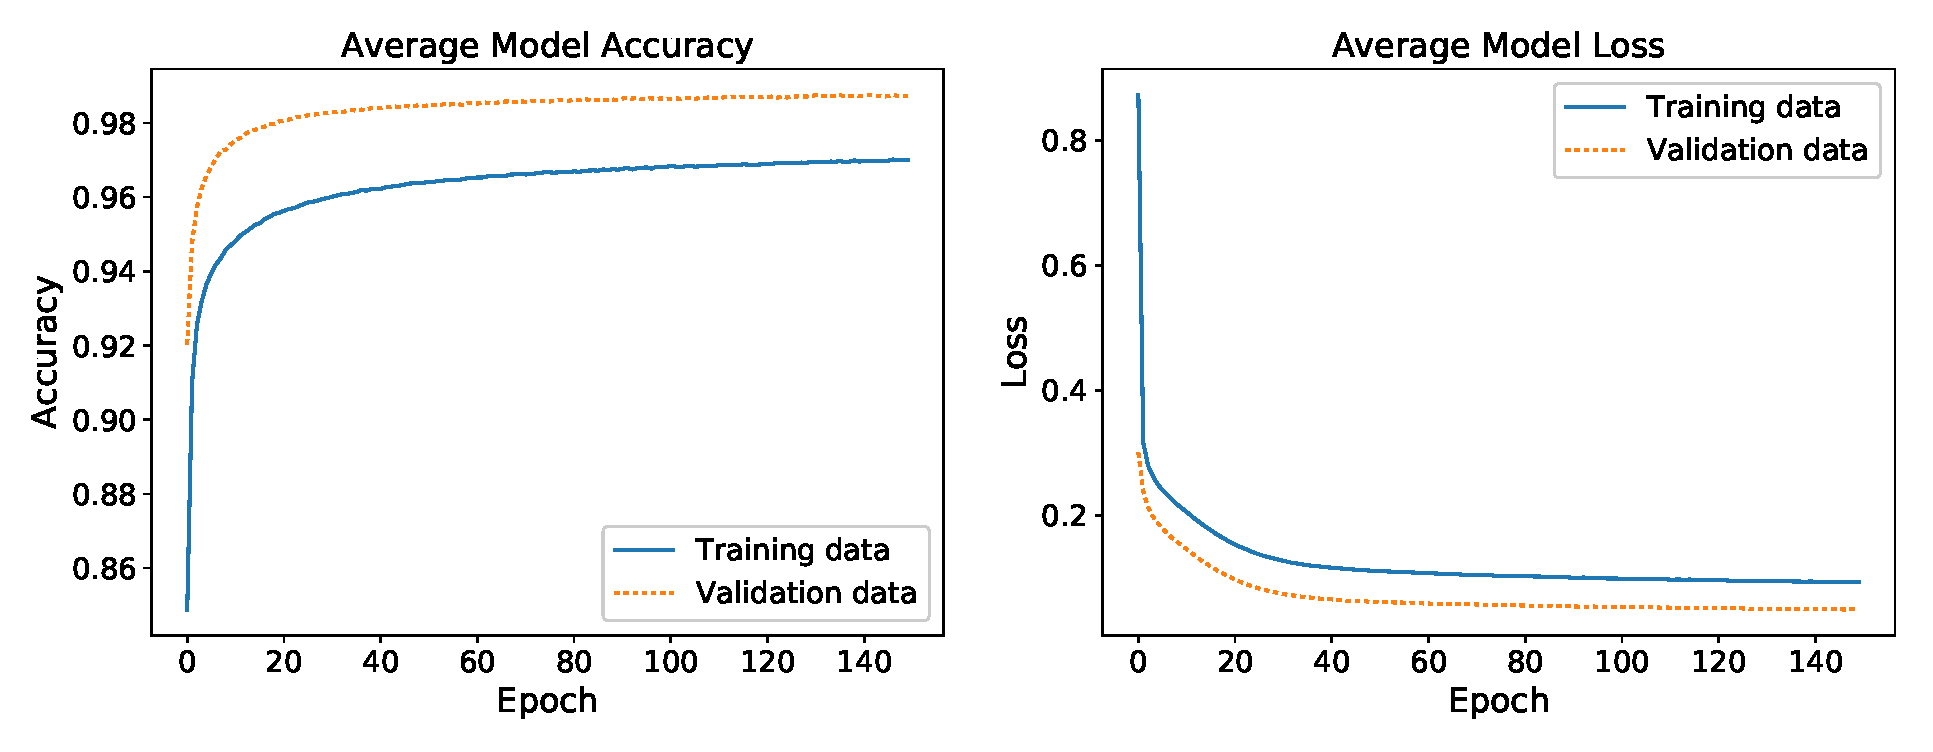
\includegraphics[width=\textwidth]{img/avg_training_metrics}
\caption{Training accuracy and loss progress on training and validation data.}
\label{fig:training_avg}
\end{figure}

To understand how well our model can emulate OSPF we need to analyze the performance on the test set; as we did for the training, we evaluate the performance of the system by averaging the results of the single models. The system achieves an average accuracy of $\textbf{98.71\%}$, with a loss of only $\textbf{0.0496}$; showing really promising results. 
%
With an accuracy of almost $99\%$, LSTM-RNNs performs better than traditional DNNs~\cite{Kato}, which achieves around 90\% of accuracy; however this comparison should be taken with caution, considered that the topologies in the two experiments are slightly different and experiments reproducibility is an open issue in machine learning~\cite{olorisade2017reproducibility}. The comparison of these two approaches is shown in Figure~\ref{fig:lstm_dnn}.

\begin{figure}[b]
\centering
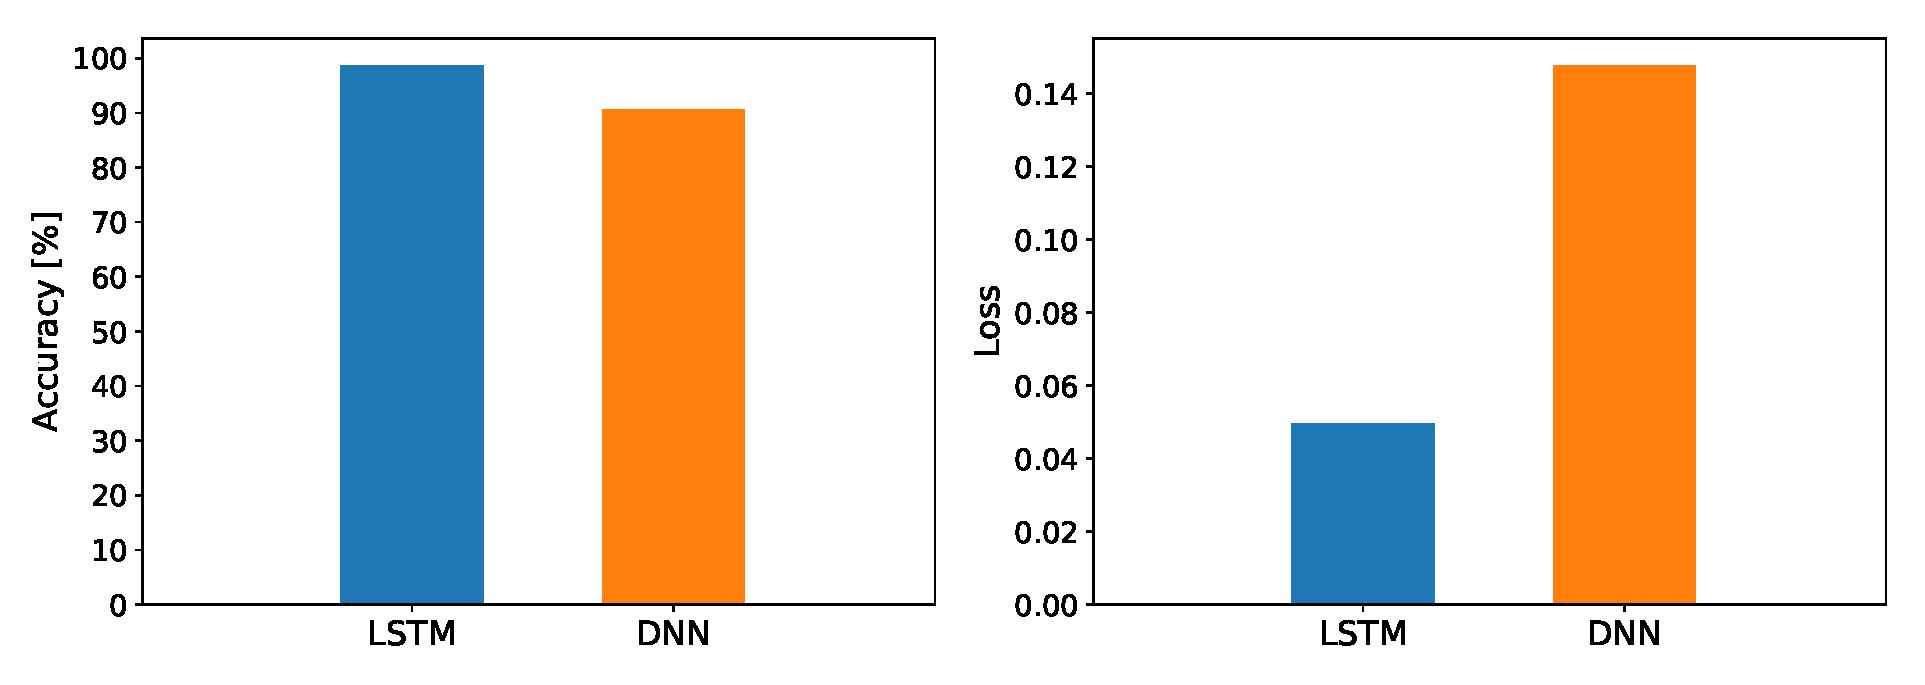
\includegraphics[width=\textwidth]{img/lstm_dnn}
\caption{LSTM and DNN performance comparison.}
\label{fig:lstm_dnn}
\end{figure}

It is important to notice that in this case, the average accuracy could be slightly misleading: the models that represent our model --- a source-destination pair connected by a single link --- are oversimplified, hence it is very likely for them to have an accuracy close to $100\%$. Nonetheless, only $32\%$ (obtained counting all directly connected targets including all the interfaces on the destination router) of the models represents this situation, that means that even if they all had $100\%$ accuracy, the remaining models would have an average accuracy of $97.89\%$.

\section{Overwriting OSPF Routing}
To evaluate our model as OSPF substitution, we observe the behavior of the path prediction system in a functioning network. 
In particular, we  use the same topology (Figure~\ref{fig:topology}) and traffic simulator adopted in the dataset generation phase; to ease the analysis process, all links are set to the same rate. Afterwards, we select a source router and a destination address and examine the difference in behavior between OSPF and our system.

In general, our system shows a dynamic behavior, predicting several paths for the same destination in different traffic conditions. More specifically, we run four traffic simulations, each of them for fifteen minutes, with a varying loss rate on the link chosen by OSPF to connect source and destination;  at the same time, the path prediction system computes a new path every five seconds. The selected target is $(R1, R3)$, with the default path being $R1,R2,R3$ and the loss being varied on the link between R1 and R2. Figure~\ref{fig:path_cmp} compares the routing decisions made by the system in comparisons: being performance unaware, OSPF always chooses the same path, even when the link has losses. Our system on the contrary, shows the ability of behaving dynamically by proposing four alternative paths.

\begin{figure}
\centering
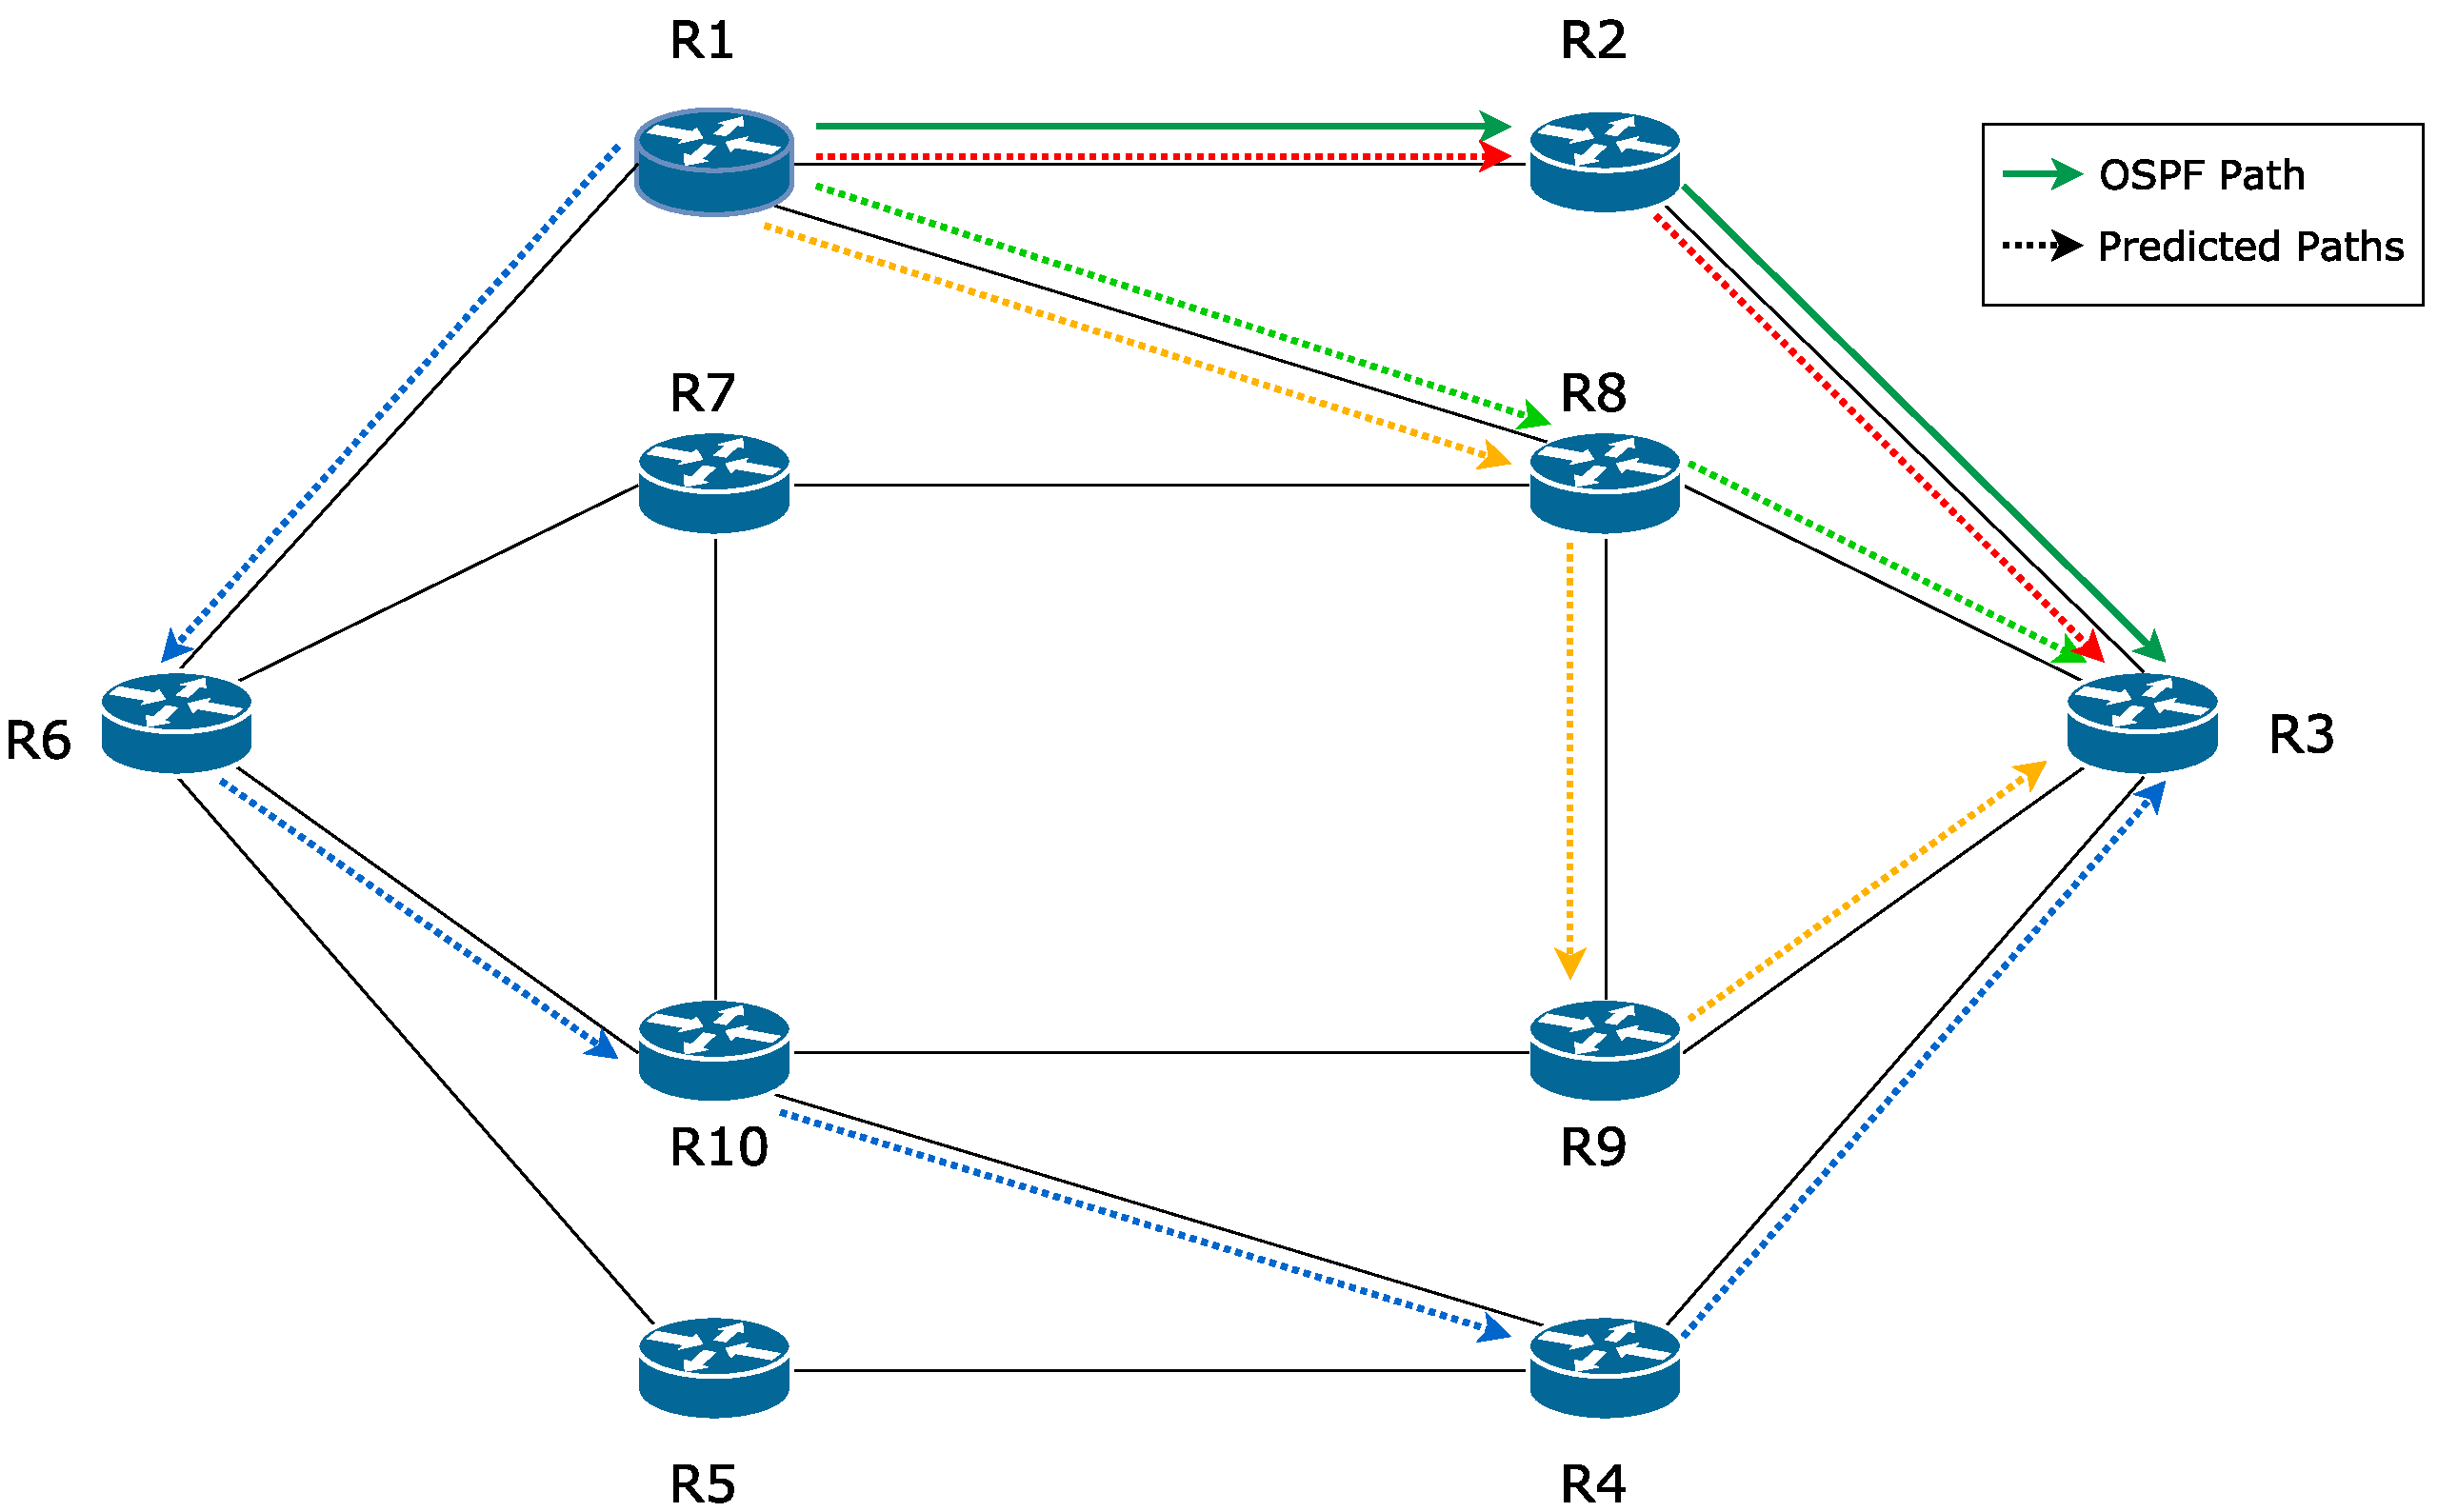
\includegraphics[width=.97\textwidth]{img/path_comparison}
\caption{Routing policies comparison.}
\label{fig:path_cmp}
\end{figure}
By studying the system behavior in presence of losses, it is possible to understand if our model is able to detect and overcome these problems. We test loss rates of 0\%, 5\%,10\%, 15\% and count the number of predictions different from OSPF (table~\ref{tab:same_path_rate}). With the loss set to $0\%$, $43\%$ of the time the predicted path is different from OSPF; if the loss is increased to $5\%$, the ratio of path different from OSPF slightly rises to $45\%$, indicating that the system is able to detect the change. The same happens for a loss of $10\%$, with a much more noticeable improvement in the system behavior;  $63.5\%$ of the proposed paths are in fact, different from the one chosen by OSPF. For the successive loss rate, equals to $15\%$, the performance goes down a little with only a $59.5\%$ different path ratio; the reasons for this loss in performance are discussed in chapter~\ref{ch:conclusion}. The ideal behavior would be for the system to detect the link loss and consequently stop predicting paths going through the damaged link. In our analysis this happens only with a limited loss rate.


Table~\ref{tab:retransmission_rate} compares the resulting retransmission rate of our system, OSPF and Equal Cost Multi Path (ECMP) routing algorithm. The retransmission rate is computed by taking into account how many times traffic would pass through the leaky link, considering two equal-cost paths for ECMP and the ratios in table~\ref{tab:retransmission_rate} for our system. Overall, the system we propose, has a lower retransmission rate than the other strategies, reaching therefore a higher throughput. Figure~\ref{fig:prediction_cmp} is a graphical comparison of the three strategies, showing the time difference needed to transmit the same amount of data. If there is no loss, the three approaches behave the same, however, as soon as a loss rate is introduced, the gap between the curves increases. This increases with the loss rate; however, while it is evident with respect to OSPF, the variation between ECMP and our system is less pronounced.

\begin{table}
\centering
{%
\begin{tabular}{|c|c|c|}
\hline
\multicolumn{1}{|l|}{\textbf{Link loss}} & \multicolumn{1}{l|}{\textbf{Different path rate}} & \multicolumn{1}{l|}{\textbf{Same OSPF path rate}} \\ \hline
0\% & 43\% & 57\% \\ \hline
5\% &45\% & 55\% \\ \hline
10\% & 63.5\% & 36.5\% \\ \hline
15\% & 59.5\% & 40.5\% \\ \hline
\end{tabular}%
}
\caption{Path predictions different and equal to OSPF.}
\label{tab:same_path_rate}
\end{table}

\begin{table}
\centering
\begin{tabular}{|c|c|c|c|c|}
\hline
\multicolumn{1}{|l|}{}  & \multicolumn{4}{c|}{\textbf{Routing Strategy}}                                          \\ \hline
\textbf{Link loss rate} & \textbf{OSPF} & \textbf{ECMP} & \textbf{DNN} &\textbf{LSTM} \\
\hline
0\% & 0\% & 0\% & 0\% & \textbf{0\%}\\
\hline
5\%  & 5\% & \textbf{2.50\%} & 2.70\%	 &2.75\%\\
\hline
10\% & 10\% & 5\% & 7.70\% & \textbf{3.65\%}\\
\hline
15\% & 15\% & 7.50\% & 9\% &\textbf{6.07\%}\\
\hline
\end{tabular}%
\caption{Routing strategies retransmission rate comparison.}
\label{tab:retransmission_rate}
\end{table}

\begin{figure}
\centering
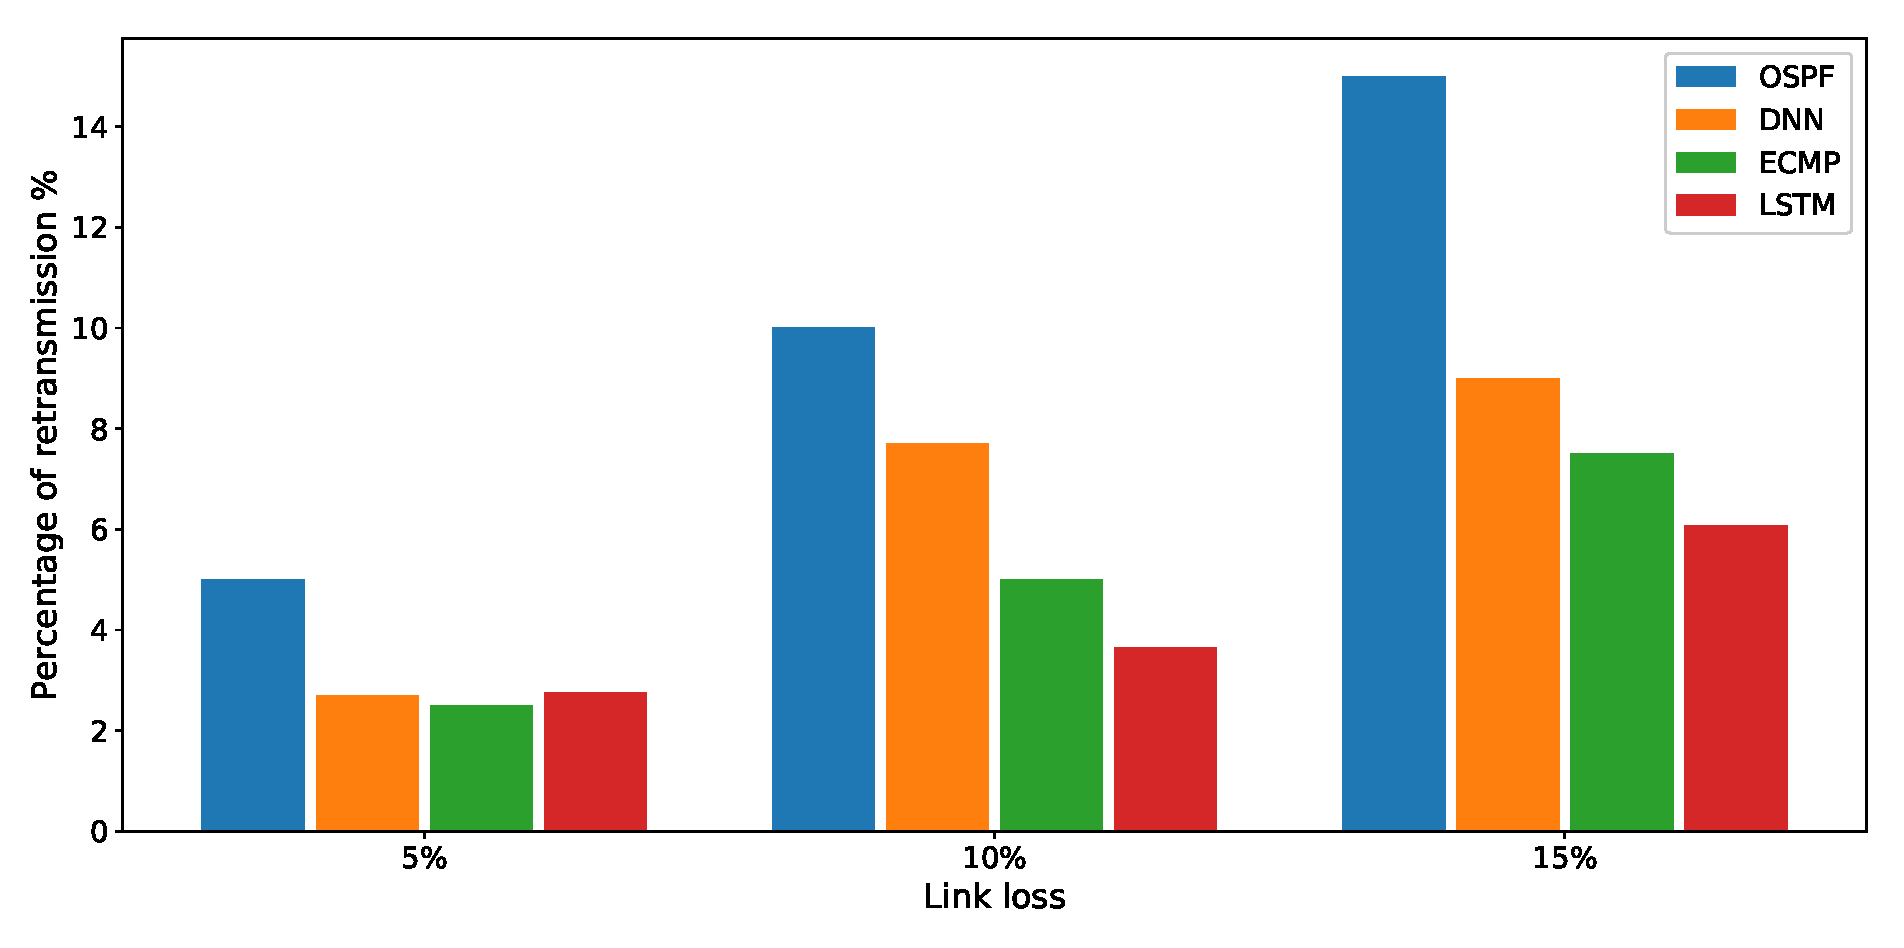
\includegraphics[width=\textwidth]{img/prediction_full_cmp_bar}
\caption{Routing policies retransmission comparison.}
\label{fig:prediction_cmp}
\end{figure}
There is another consideration that needs to be made when talking about OSPF. It would be unfair to consider this protocol completely performance unaware; during our tests, we have noticed that starting from a certain point, OSPF is  able to detect the problem. In our case, with a link loss greater than or equal to $20\%$, OSPF changes its output, selecting a new shortest path. This behavior is caused by the fact that when the loss on the link is too high, the HELLO (i.e., keep-alive) packets used by the protocol are lost, causing the link discovery part of the algorithm to deviate to other routes. We believe that this is a Mininet's limitation and its way to interpret the loss as a fixed phenomenon happening on the link. We know that in real networks losses don't work this way, therefore we are limited in the testing possibilities; nonetheless these results look promising.

\section{A critical scenario}
To have a more clear idea about our system capabilities, we test it in a critical scenario. We decide to simulate a network in which statistically, half of the links are affected by a loss rate; we test the same loss rates of the previous experiments ($5\%$, $10\%$, $15\%$), ten times each, generating traffic between five different targets. The purpose of this experiment is to understand if our system can tolerate better than OSPF a condition where half of the network is not functioning properly. To compare the performance of the two approaches we counted the number of times the links with loss were used; the results are shown in Figure~\ref{fig:stress_test}. The chart compares the total number of defective links traversed in all the runs for each link loss rate. From the results, it appears that our proposed system does not introduce any significant advantage under critical circumstances; the chart shows in fact, that overall, the performance of the two systems are similar, with OSPF performing better when the link loss rate is set to $10\%$ and $15\%$. The reasons of these poor performance are to be found in how our system works: we trained our model to predict alternative paths based on the network conditions; even in this case, the proposed system is able to suggest alternative paths. The main problem is that, given that half of the link in the networks is affected by a loss, the majority of the proposed alternative paths passes through these links, resulting in poor performance. In the conclusions (chapter~\ref{ch:conclusion}) we give a few hints on how to overcome such limitations of our system.

\begin{figure}
\centering
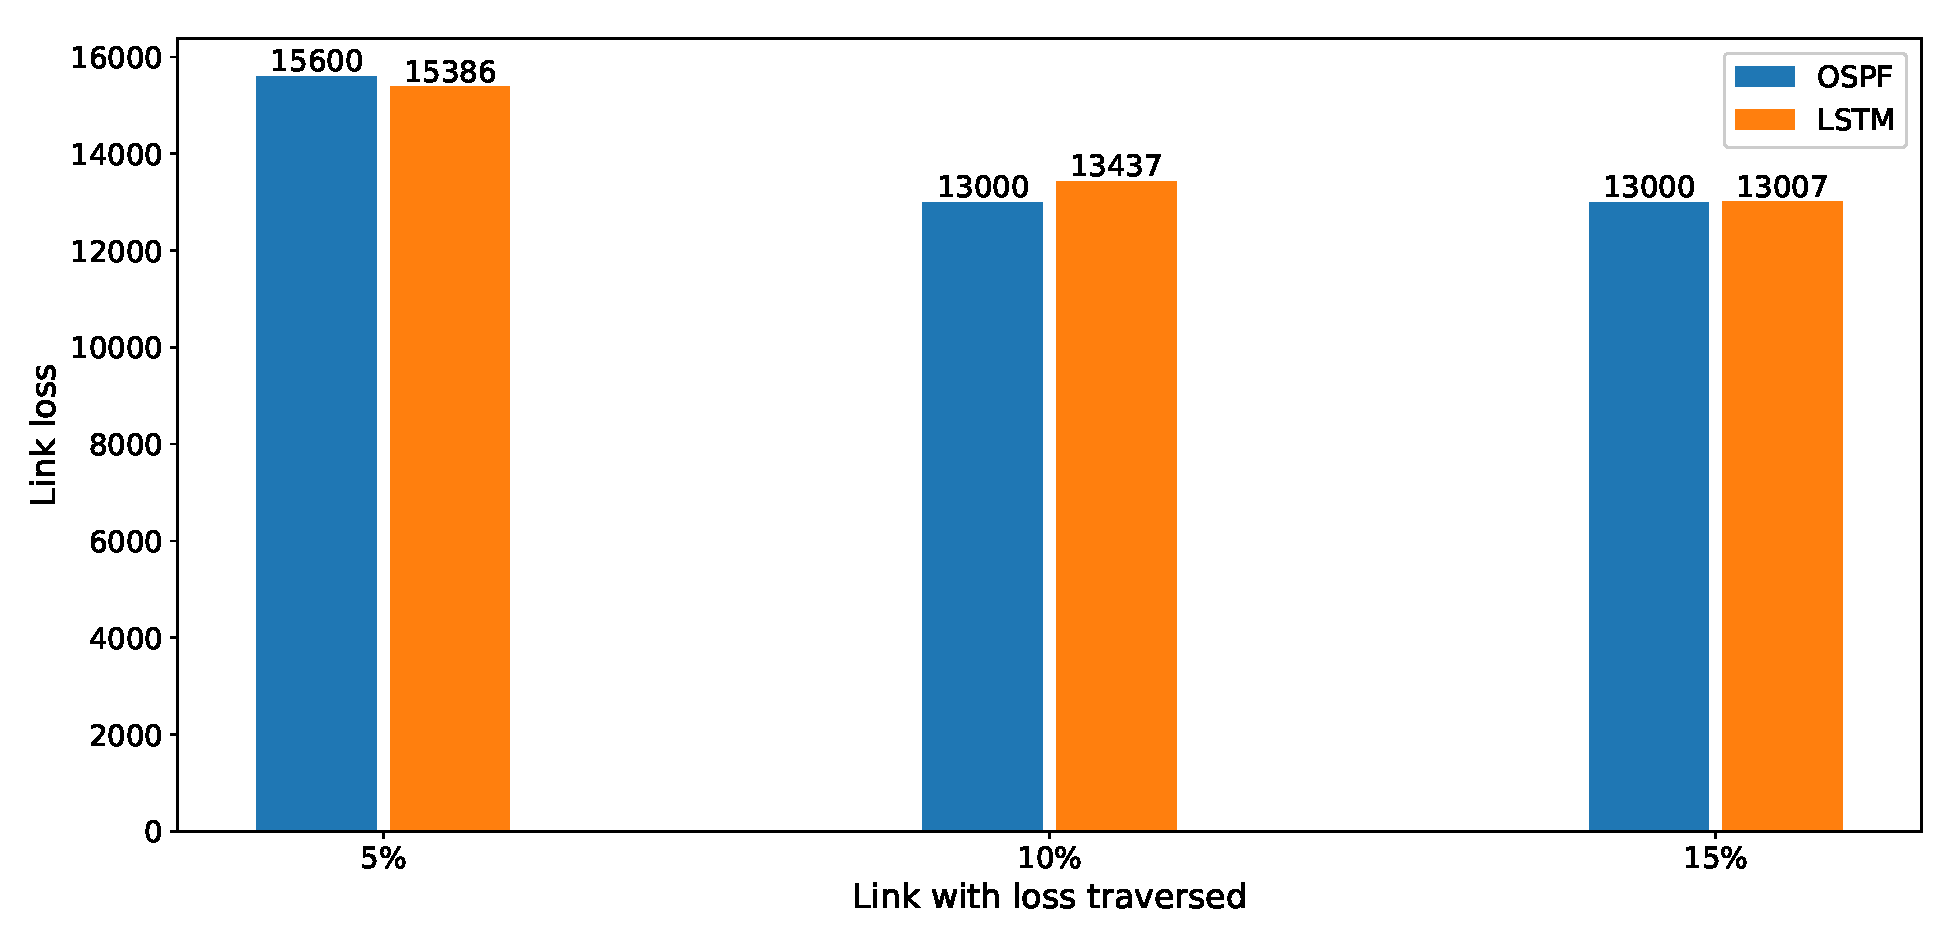
\includegraphics[width=0.949\textwidth]{img/stress_test}
\caption{Comparison of the number of (severely) lossy links traversed by OSPF and LSTM.}
\label{fig:stress_test}
\end{figure}

\chapter{Conclusions and Results}

Lorem ipsum dolor sit amet, consectetur adipiscing elit, sed do eiusmod tempor incididunt ut labore et dolore magna aliqua. Ut enim ad minim veniam, quis nostrud exercitation ullamco laboris nisi ut aliquip ex ea commodo consequat. Duis aute irure dolor in reprehenderit in voluptate velit esse cillum dolore eu fugiat nulla pariatur. Excepteur sint occaecat cupidatat non proident, sunt in culpa qui officia deserunt mollit anim id est laborum.
\cleardoublepage
\nomenclature{\textbf{RNN}}{Recurrent Neural Network}
\nomenclature{\textbf{AI}}{Artificial Intelligence}
\nomenclature{\textbf{ML}}{Machine Learning}
\nomenclature{\textbf{LSTM}}{Long Short-Term Memory}
\nomenclature{\textbf{CNN}}{Convolutional Neural Network}
\nomenclature{\textbf{SDN}}{Software-Defined Networking}
\nomenclature{\textbf{KDN}}{Knowledge-Defined Networking}
\nomenclature{\textbf{OSPF}}{Open Shortest Path First}
\nomenclature{\textbf{ECMP}}{Equal Cost Multi-Path}
\nomenclature{\textbf{DNN}}{Deep Neural Network}
\nomenclature{\textbf{NN}}{Neural Network}
\nomenclature{\textbf{KP}}{Knowledge Plan}
\nomenclature{\textbf{iBGP}}{Internal Gateway Protocol}
\nomenclature{\textbf{BGP}}{Border Gateway Protocol}
\nomenclature{\textbf{eBGP}}{External Protocol}
\nomenclature{\textbf{IP}}{Internet Protocol}
\nomenclature{\textbf{IoT}}{Internet of Things}
\nomenclature{\textbf{ISP}}{Internet Service Provider}
\nomenclature{\textbf{RL}}{Reinforcement Learning}








%now enable appendix numbering format and include any appendices
\appendix
\chapter{Sample Title}

Lorem ipsum dolor sit amet, consectetur adipiscing elit, sed do eiusmod tempor incididunt ut labore et dolore magna aliqua. Ut enim ad minim veniam, quis nostrud exercitation ullamco laboris nisi ut aliquip ex ea commodo consequat. Duis aute irure dolor in reprehenderit in voluptate velit esse cillum dolore eu fugiat nulla pariatur. Excepteur sint occaecat cupidatat non proident, sunt in culpa qui officia deserunt mollit anim id est laborum.
\chapter{Sample Title}

Lorem ipsum dolor sit amet, consectetur adipiscing elit, sed do eiusmod tempor incididunt ut labore et dolore magna aliqua. Ut enim ad minim veniam, quis nostrud exercitation ullamco laboris nisi ut aliquip ex ea commodo consequat. Duis aute irure dolor in reprehenderit in voluptate velit esse cillum dolore eu fugiat nulla pariatur. Excepteur sint occaecat cupidatat non proident, sunt in culpa qui officia deserunt mollit anim id est laborum.

\end{document}

